\documentclass[10pt]{beamer}

% Theme and color scheme
\usetheme{Madrid}
\usecolortheme{default}

% packages
\usepackage{amsmath}
\usepackage{calc}
\usepackage{tikz}
\usetikzlibrary{arrows.meta,positioning,calc}
\usepackage[normalem]{ulem}

% Title page information
\title[Linear and Nonlinear KF]{Linear and Nonlinear Kalman Filtering: theory and applications}
\subtitle{SCUDO/DAUSY/DRIM Ph.D. course A.Y. 2026}
\author{Marco Todescato}
\institute[FHI]{Fraunhofer Italia Research SCARL}
\date{\today}

% to remove nav symbols
% \setbeamertemplate{navigation symbols}{}


\newcommand{\myframe}[2]{%
\begin{frame}%
    \frametitle{#1}%
    #2%
\end{frame}
}

\newcommand{\sectionframe}[2]{%
\begin{frame}[c]%
    \centering
        \begin{enumerate}
            \setcounter{enumi}{\numexpr#1-1\relax}
            \item \textcolor{blue}{#2} 
        \end{enumerate}%
\end{frame}
}

% def
\newcommand{\tq}[1]{\textquotedblleft#1\textquotedblright}

%maths
\newcommand{\inner}[2]{\langle#1,#2\rangle}
\newcommand{\spn}[1]{\operatorname{span}\left\{#1\right\}}
\newcommand{\clspn}[1]{\overline{\operatorname{span}}\left\{#1\right\}}
\newcommand{\until}[1]{\left\{1,\ldots,#1\right\}}
\newcommand{\cls}[1]{\operatorname{cls}\left\{#1\right\}}
\newcommand{\Hpast}[1]{\H^{-}_{#1}}
\newcommand{\Hfuture}[1]{\H^{+}_{#1}}

\newcommand{\todo}[1]{\textcolor{red}{TODO: #1}}

% \customblock{type}{title}{content}  %snapping block to content size
\newcommand{\customblock}[3]{%
    \begin{center}
        \begin{minipage}{\widthof{#3}+.5cm}
            \begin{#1}{#2}
                \centering
                #3
            \end{#1}
        \end{minipage}
    \end{center}
}



% math
\def\Z{\mathbb{Z}}
\def\C{\mathbb{C}}
\def\E{\mathbb{E}}
\def\Elin{\hat{\mathbb{E}}}
\def\R{\mathbb{R}}
\def\S{\mathcal{S}}
\def\A{\mathcal{A}}
\def\x{\mathbf{x}}
\def\xhat{\hat{\x}}
\def\xerr{\tilde{\x}}

\def\y{\mathbf{y}}
\def\yhat{\hat{\y}}
\def\yerr{\tilde{\y}}

\def\w{\mathbf{w}}
\def\what{\hat{\w}}
\def\werr{\tilde{\w}}

\def\z{\mathbf{z}}
\def\zhat{\hat{\z}}
\def\zerr{\tilde{\z}}

\def\v{\mathbf{v}}
\def\vhat{\hat{\v}}
\def\verr{\tilde{\v}}

\def\r{\mathbf{r}}

\def\u{\mathbf{u}}
\def\n{\mathbf{n}}
\def\p{\mathbf{p}}
\def\e{\mathbf{e}}
\def\a{\mathbf{a}}
\def\xiv{\mathbf{\xi}}
\def\X{\mathbf{X}}
\def\mux{\mu_{\x}}
\def\muy{\mu_{\y}}
\def\muz{\mu_{\z}}
\def\N{\mathcal{N}}
\def\muzero{\mu_{0}}
\def\Pzero{P_0}
\def\xzero{\x_0}
\def\Varzero{\Sigma_{0}}
\def\Varx{\Sigma_{\x}}
\def\Vary{\Sigma_{\y}}
\def\Varz{\Sigma_{\z}}
\def\Var{\textnormal{Var}}
\def\Cov{\textnormal{Cov}}
\def\H{\textnormal{\textbf{H}}}



% \setlength{\parskip}{10pt}

\begin{document}

% Title frame
\myframe{}{\titlepage}

% outline
\myframe{Outline}{\tableofcontents}


% SECTIONS

%%%%%%%%%%%%%%%%%%%%%%%%%%%%%%%%%%%%%%%%%%%%%%%%%%%%%%%%%%%%%%%%%%%%%%%%%%%%%%%%
\section{General info about the course and Introduction}
\sectionframe{1}{General info about the course and Introduction}

%--------------------------
\myframe{Schedule}{
    \begin{tabular}{c|c|l}
        \textbf{Date} & \textbf{Time} & \textbf{Tentative Topic}\\
        Mon. 27/04/2026 & h10.30-12:30 (2h) & Intro e Preliminaries\\
        Mon. 04/05/2026 & h09.30-12:30 (3h) & Preliminaries/Linear Theory\\
        Mon. 11/05/2026 & h09.30-12:30 (3h) & Linear Theory\\
        Mon. 18/05/2026 & h09.30-13:30 (4h) & Linear Theory + Essay\\
        Mon. 25/05/2026 & h09.30-13:30 (4h) & Linear/Nonlinear Theory + Essay\\
        Mon. 01/06/2026 & h09.30-13:30 (4h) & Nonlinear Theory/Adds-on + Essay 
    \end{tabular}

    \vspace{.5cm}
    \pause
    \begin{tabular}{c|c|l}
        \textbf{Date} & \textbf{Time} & \textbf{Tentative Topic}\\
        Mon. 27/04/2026 & h10.30-12:30 (2h) & Intro e Preliminaries\\
        \sout{\textcolor{red}{Mon. 04/05/2026}} & \sout{\textcolor{red}{h09.30-12:30 (3h)}} & Preliminaries/Linear Theory\\
        Fri. 08/05/2026 & h10.30-13:30 (3h) & \\
        Mon. 11/05/2026 & h09.30-12:30 (3h) & Linear Theory\\
        \sout{\textcolor{red}{Mon. 18/05/2026}} & h09.30-13:30 (4h) & Linear Theory + Essay\\
        Fri. 15/05/2026 &  & \\
        \sout{\textcolor{red}{Mon. 25/05/2026}} & h09.30-13:30 (4h) & Linear/Nonlinear Theory + Essay\\
        Fri. 22/05/2026 & h09.30-13:30 (4h) & Linear/Nonlinear Theory + Essay\\
        \sout{\textcolor{red}{Mon. 01/06/2026}} & h09.30-13:30 (4h) & Nonlinear Theory/Adds-on + Essay\\
        Mon. 25/05/2026 & h09.30-13:30 (4h) & Nonlinear Theory/Adds-on + Essay 
    \end{tabular}
}

%--------------------------
\myframe{Exam}{
    % \begin{enumerate}
    %     \setcounter{enumi}{\numexpr1-1\relax}
    %     \item Proofs of theorems seen during lessons 
    %     \begin{itemize}
    %         \item during lessons we will encounter some (few) basic
    %         theorems/corollaries/properties. You are asked \underline{\textbf{to
    %         try}} to prove them formally on your own.
    %         \item do your best and try not to cheat!
    %         \item you can work in a group if preferred. 
    %     \end{itemize}
    % \end{enumerate}
    % \vspace{0.2mm}
    % AND
    % \vspace{0.2mm}
    % \begin{enumerate}
    %     \setcounter{enumi}{\numexpr2-1\relax}
    %     \item Practical coding essay:
    %     \begin{itemize}
    %         \item on a selected application: pick a topic that is relatable to
    %         your need/research.
    %         \item partially developed during class.
    %         \item programming language: python (MATLAB is an option but try to
    %         avoid it), either using jupyter notebook or script based. Make sure all
    %         necessary dependencies to run are available.
    %         \item no use of predefined libraries with KF implementations.
    %         \item you can work in a group if preferred.
    %         \item \underline{\textbf{objective}:} explore (possibly all) the
    %         topics covered during the course, from linear to non-linear KF. You
    %         might need to start from modeling assumptions, linearize if
    %         necessary, discuss noise statistics and then implement the filter.
    %         Try to explore limits and nuances as if it were a small research
    %         project.
    %     \end{itemize}
    % \end{enumerate}

    Practical coding essay + report:
        \begin{itemize}
            \item on a selected application: pick a topic possibly related to
            your need/research.
            \item partially developed during class.
            \item programming language: python -- either using jupyter notebooks
            (recommended) or script based. Make sure all necessary dependencies
            to run are available.\\\textbf{For other programming language ask first!!}
            \item no use of predefined libraries with KF implementations.
            \item you can work in a group if preferred.
            \item \underline{\textbf{objective}:} explore (possibly all) the
            topics covered during the course, from linear to non-linear KF. You
            might need to start from modeling assumptions, linearize if
            necessary, discuss noise statistics and then implement the filter.
            Try to explore limits and nuances as if it were a small research
            project.
            \item present results in a pdf report\footnote{For well organized
            runnable Jupyter notebooks this is optional. If, upon agreement,
            another language is used this is mandatory.}
        \end{itemize}

}

%--------------------------
\myframe{References and additional material}{
    \begin{itemize}
        \item [IT] \textbf{Picci, G. (2007). Filtraggio statistico (Wiener, Levinson, Kalman) e applicazioni. Libreria Progetto.}
        \item [EN] Sanso F., Pileggi, C. and Biagi, L. (2024). A tutorial on Kalman filtering. The linear, extended and unscented filters. (pdf available as resource in the material folder)
        \item [EN] Anderson, B. D., and Moore, J. B. (2005). Optimal filtering. Courier Corporation.
    \end{itemize}

    \vspace{5mm}

    G-drive:\\
    {\small
    \url{https://drive.google.com/drive/folders/1BbuSTiO4wym0qOAqeLUkiVum_14kRRzD}}

    \vspace{5mm}

    github: for complete slides, code and additional resources\\
    {\small
    \url{https://github.com/MarcoTodescato/linear_and_nonlinear_kalman_filtering}}

    \vspace{5mm}
    For Q/A and discussion we can set up a Discord channel
}


%--------------------------
\myframe{Goal}{%
How to formulate estimation problems encountered in many engineering fields and
applications as instances of a general dynamical system state estimation problem
and how to derive the mathematical solution of the latter problem (possibly
depending on additional assumption on the functional family of the considered
dynamical system).%

\vspace{10mm}

\pause
\textbf{Essentially, this will lead to the well-known (linear) Kalman filter and
its (nonlinear) extensions.}%
}

%--------------------------
\myframe{A bit of history: the theories of statistical filtering}{%

\begin{exampleblock}{Wiener-Kolmogorov (1940)}
    \begin{itemize}
        \item $I=(-\infty, t]$, infinite time support
        \item $\{\x(t)\}$, $\{\y(t)\}$ are weakly jointly stationary
    \end{itemize}
    The impulse response of the optimal filter is time-invariant hence it can be
    analytically computed once and for all times, knowing the processes
    statistics.
\end{exampleblock}

\pause

\begin{block}{Levinson (1950)}
    \begin{itemize}
        \item no more infinite (lower unbounded) time support
    \end{itemize}
    The impulse response of the filter is time-varying but can be efficiently
    computed at time $t$ using a recursive structure which exploits the
    computations until $t-1$. 
\end{block}

\pause

\begin{alertblock}{Kalman (1960)}
    \begin{itemize}
        \item signals can be modeled as stochastic dynamical systems of finite
        size
    \end{itemize}
    Looks for recursive finite-memory schemes that resembles that same dynamical
    system structure of finite size.
\end{alertblock}
}

%--------------------------
\myframe{A bit of history: a change of perspective}{%
Revolutionary apporach introduced by R.E. Kalman in 1960 to the problem of
statistical filtering.%

\vspace{5mm}

Change of perspective:
\begin{itemize}
    \item \textbf{Wiener-Kolmogorov}: explicit computation of the filter
    \textbf{transfer function}, practically useful only for signals
    characterized by a \textbf{rational} spectral density
        \begin{itemize}
            \item implicit computations possible only for rational signals
            \item actual physical implementation of the filter as a set of
            difference (recursive) equations only for rational representations
        \end{itemize}

    \pause
    \medskip
    \item \textbf{Kalman}: hypothesis that the signals can be described as
    (linear) \textbf{dynamical systems} of finite dimension
        \begin{itemize}
            \item no transfer functions involved
            \item natural formulation of the filter as a fixed algorithmic
            structure essentially consisting of a discrete-time (linear)
            dynamical system of finite memory, driven by measurements
            \item implementation always possible as a recursive algorithm 
        \end{itemize}
\end{itemize}
}

%--------------------------
\myframe{Prediction vs Filtering vs Smoothing}{%
Assume $\{\x(t)\}$ and $\{\y(t)\}$ are (second order\footnote{First and second
moment statistics exist and are finite.}) processes of known dimensions. Denote
with $\xhat(t|I)$ the estimator of $\x(t)$ given $\{\y(t)\}_{t\in I}$, $I$ being
the time support.

\vspace{.2cm}

It is possible to identify 3 classes of \underline{\textbf{estimation problems}}.

\vspace{.2cm}

\pause
\begin{block}{Prediction}
    Find $\xhat(t+h|I)$ being $I=[t_0,t]$ and $h>0$, that is the estimator
    $h$-step ahead in the future from measurements up to time $t$.
\end{block}

\pause
\begin{block}{Filtering}
    Find $\xhat(t|I)$ being $I=[t_0,t]$, that is the estimator at current time
    $t$ from all available measurements up to $t$. 
\end{block}

\pause
\begin{block}{Smoothing}
    Find $\xhat(t|I)$ being $I=[t_0,t_1]$ with $t<t_1$, that is the estimator at
    time $t$ from all available measurements up to $t_1$ in the future.
\end{block}
}


\section{Preliminaries}
\sectionframe{2}{Preliminaries: before diving in... some definitions and preliminary results}

%--------------------------
\myframe{Random signals and stochastic processes}{%

\begin{block}{Random signal}    
    A random signal can defined as the tuple $(T,V,S)$ where
    \begin{itemize}
        \item $T$ is the set of time. We consider discrete-time signals, $T=\Z$
        \item $V$ is the \tq{alphabet} of signal values, $V=\R$ or $V=\R^n$
        \item $S$ is the sample space. Every $s\in S$ is a function $s:t\mapsto s(t)$
        where $t\in T$ and $s(t) \in V$ also called \textit{trajectory} of the signal
    \end{itemize}
\end{block}

\pause

\begin{block}{Stochastic process}
    Mathematical formulation/description used to formally model the aleatoric
    nature of a random signal. Consisting of the tuple $(S,\S, P)$ where:
    \begin{itemize}
        \item $S$ sample space. Set of all possible trajectories
        \item $\S$ events set of all logical propositions or events regarding the signal
        \item $P$ probability measure on $\S$, i.e. $P: \S\mapsto [0,1]$ mapping
        every $A\in\S$ to $P(A)\in[0,1]$, the a-priori
        \tq{confidence} $A$ actually happening
    \end{itemize}
\end{block}
}


%--------------------------
\myframe{A more general formulation}{%

\begin{block}{Stochastic process (usual def in prob. theory)}
    A collection of random variables, $\{y(t)\}$, indexed by a temporal index
    $t\in T$, all defined on the same (abstract) probability space $(\Omega, \A,
    P)$ where:
    \begin{itemize}
        \item $\Omega$ event set of \tq{state of nature} $\omega$
        \item $\A$ $\sigma$-algebra of subsets of $\Omega$ 
        \item P probability measure on $\A$
    \end{itemize}
    Each variable is a ($\A$-measurable) function $y(t): t \mapsto y(t,\omega)$. The
    \textit{trajectories} are the successive determinations
    $\{y(\cdot,\tilde{\omega})\}$ of $y(t)$ corresponding to a particular event
    $\tilde{\omega}\in\Omega$
\end{block}

\pause

Our definition $(S,\S,P)$ is a \tq{concrete} version of the abstract
$(\Omega,\A,P)$. If we define a variable
$y(t)\in(S,\S,P)$ as
%
$$
y(t,s) := s(t)
$$
where $y(t)$ associates at every trajectory $s\in S$ its value at $t$, then it
is clear that, for varying $t$, the successive determinations of the variables
$\{y(t)\}$ corresponding to the event $\overline{s}\in \S$ describe indeed the
trajectory $\{\overline{s}(t)\}$ of the process.
}

%--------------------------
\myframe{Let's clarify...}{%

The probabilistic formulation and formalization introduced is \textit{just} a
convenient choice to describe (or model) the unpredictable nature of a signal.
It is worth remembering that this is one possible choice that eventually
allows one to resort to tools from probability theory to describe, handle and
develop useful tools for filtering and identification. For this reason, it is
important to understand that, regardless the real nature of the underline
signal, the same formulation (as \textit{stochastic process}) can indeed be used
to describe every signal (aleatoric or not). On the other hand, it might be
worth remembering that this choice is dictated by the \tq{simplicity},
compactness and generality to describe events that could indeed also be
described using a \tq{deterministic} formulation.
}

%--------------------------
\myframe{The Problem of \textit{Estimation}: Estimate vs Measure}{%

Statistical problem of estimation seen as formalization of the mathematical
problem of measuring where the goal is that of getting information about a
desired quantity $x$, non directly observable, based on observable data, $y$,
whose values are produced by the measurement \tq{instrument}.

\vspace{3mm}

\pause
Ideally, knowing the \tq{physical coupling}, i.e., relation, between $x$ and
$y$ should allow to retrieve the value of $x$ based on observable values of
$y$. Practically, this relation is either not perfectly known or influenced
by \textit{environmental conditions} which introduce \textit{uncertainty} in
the measurement process.

$$
y=h(x) \Longleftrightarrow y=h(x) + \epsilon
$$

As a consequence, the objective can be understood (or interpreted) as that
of \textit{estimating} the value of $x$ based on the observed values of $y$.

\vspace{3mm}

\pause
Following this \tq{uncertainty-based} interpretation:
\begin{itemize}
    \item it is not always straightforward how to generally get $x$ from $y$
    \item being impractical (meaningless) to reconstruct $x$ with certainty, how
    to \textit{best} approximate it? 
\end{itemize}
}

%--------------------------
\myframe{The Bayesian approach}{%

\begin{block}{}
    $x$ assumed to be a random quantity characterized by some a-priori
    information
\end{block}

\pause

\begin{alertblock}{Notation: random variables vs sample values}
    It is important to understand the difference between a random variable, for
    which bold letters $\x$ will be used vs the corresponding sample values,
    i.e., the actual value taken by the random variable, for which normal case
    letters $x$ will be used.
\end{alertblock}

\pause

\begin{block}{Bayesian inference}
    Assume there exist a random variable/vector $\x$ described by the
    probability density $p_\x(x)$ and the random variable/vector $\y$ of
    measurements described by the conditional density $f(y|x) = f(y|\x=x) =
    \frac{P(y\leq \y \leq y+dy | \x=x)}{dy}$.
    
    \vspace{3mm}

    The problem of Bayesian inference/estimation is that of reconstructing $\x$
    based on $p_\x$, $f(y|x)$ and the observation of $\y=y$. This can be
    understood as to:
    \begin{itemize}
        \item compute the new distribution of $\x$ determined by the observation $\y=y$, or
        \item reconstruct $x=\x(\omega)$ determined by the \tq{measurement}
        process
    \end{itemize}
\end{block}
}

%--------------------------
\myframe{Bayesian inference: complete reconstruction}{%
Assuming $p_\x(x)$ and $f(y|x)$ completely known, the problem is that of
computing

$$
f(x|y) = \frac{f(y|x)p_\x(x)}{\int f(y|x)p_\x(x) dx} = \frac{p_{\y\x}(y, x)}{p_\y(y)}
$$

i.e., the conditional \textit{a-posteriori} density of $\x$ given $\y=y$, which
is the most exhaustive and complete description possible.

\vspace{5mm}

\pause

Explicit analytical computation of the above equations often not possible.

\vspace{5mm}

\pause

In practice, this is rarely the case and/or even necessary because rather than
an exhaustive description, a more handy point estimate of $\x$, telling us what
is the unobservable sample value $\x=x$ that gave rise to the observation
$\y=y$, is more useful.

}

%--------------------------
\myframe{Bayesian inference: point estimate}{%

Assume the relation between $\x$ and $\y$ could analytically be described as

$$
\y = h(\x, \w)
$$

being $\w$ the random vector capturing the variable interations with the
environment, i.e., the \tq{measurement noise}. 

\vspace{5mm}

\pause

During the measurement process the particular experimental conditions $\omega$
give raise to a specific determination $\w(\omega)=w$ which, in turn, give raise
to an observed value $\y=y$ linked to $\x=x$ by the relation

$$
y=h(x,w)
$$

\pause

Then, the problem is that of reconstructing the value $x$ of $\x$ that
\tq{caused} $\y=y$ during the measurement process. Since estimating/knowing $w$
is intrinsically impossible, the problem is understood as that of \tq{best}
approximating $x$.

\vspace{3mm}

\pause

It is then necessary to define a \tq{reasonable} class of approximation criteria.
}

%--------------------------
\myframe{Bayesian inference: conditional/posterior expected risk}{%

\begin{block}{Cost/Loss Function}
    It is called \tq{loss/cost} a scalar function $c: \R^n\mapsto\R$ of $\xi=z-x$,
    $z\in\R^n$, s.t. $c\geq0$, $c''>0$ (strictly convex) and $c(0)=0$. It is said
    symmetric if $c(-\xi)=c(\xi)$.

    \vspace{3mm}

    E.g.: $c(z-x)=\|z-x\|^2_Q$ where $Q>0$ symmetric and $\|x\|^2_Q = x^TQx$.
\end{block}

\pause
$z$ plays the role of approximation of $x$. The problem could then be that of
finding $z$ that minimizes $c$ for every value of the unknown $x$. In practice
it is \tq{smarter} to consider all the available probabilistic information,
e.g., given by $\y=y$.

\pause
\begin{block}{Conditional Expected Risk and Point Bayesian Estimate}
    Consider the \textit{Conditional Expected Risk}
    $$
    R(z,y):=\E[c(z-\x)|\y=y]= \int_{\R^n} c(z-x)f(x|y)dx
    $$
    Then, the \textit{Point Bayesian Estimate} is defined as
    $$
    \hat{x}= \textnormal{Arg min}_z R(z,y)
    $$
\end{block}
}

%--------------------------
\myframe{Bayesian inference: Conditional Expectation}{%

\begin{exampleblock}{Theorem: Conditional Expectation}
    If the loss $c$ is symmetric and the conditional density $f(\cdot|y)$ is
    symmetric around its mean $\mu(y)=\E[\x|\y=y]=\int xf(x|y)dx$, then
    $\hat{x}$ does not depend on $c$ and it is equal to the conditional mean of
    $\x$ given $\y=y$, i.e., $\E[\x|\y=y]$.

    \vspace{3mm}

    Moreover, if the cost $c$ is of quadratic form, i.e., $\|\cdot\|^2_Q$, then
    $\hat{x}=\E[\x|\y=y]$ for all types of conditional density $f(x|y)$
    (assuming the conditional mean exists).

    \vspace{3mm}

    More generally, among all possible measurable functions $g:
    \R^m\mapsto\R^n$, for every symmetric $Q>0\in \R^{n\times n}$, 
    % the conditional mean $\E[\x|\y]$ is that minimizing the
    % mean of the squared distance $\|\x-g(\y)\|_Q$, i.e.,
    $$
    \E[\x|\y] = \textnormal{Arg min}_{g(\cdot)} \E[\|\x-g(\y)\|_Q^2]
    $$
\end{exampleblock}

\vspace{1mm}

\pause

Interpreted as a function of $y$, for symmetric $c$ and $f$, the conditional
mean $\E[\x|\y]: y \mapsto \E[\x|\y=y]$ is the Bayesian
estimator\footnote{Estimator: function (algorithm) of the observed data mapping
them to point estimates.} $\hat{x}$ of $x$ that minimizes the conditional
expected risk $R(z,y)$. This is also true for any $f$ if $c$ is quadratic. In
this case it is referred to as the \textit{minimum squared Bayesian estimator}. 
}

%--------------------------
\myframe{Theorem: Conditional Expectation (proof of last part)}{%

For the law of total expectation, we can write
%
\begin{align*}
    \E[\|\x-g(\y)\|_Q^2] &= \int_\R p_\y(y) \E[\|\x-g(\y)\|_Q^2 | \y = y]dy \\
                         &= \E\left[
                                \E[ \|\x-g(\y)\|_Q^2 | \y ]
                               \right] \\
                         &= \E\left[
                                \E[ \|\x - \E[\x|\y] + \E[\x|\y] - g(\y)\|_Q^2 | \y ]
                              \right] \\
                         &= \E\Big[
                                   \E[ [\x - \E[\x|\y]]^T    Q [\x - \E[\x|\y]]    | \y ] \\
                         &\quad + 2\E[ [\x - \E[\x|\y]]^T    Q [\E[\x|\y] - g(\y)] | \y] \\
                         &\quad +  \E[ [\E[\x|\y] - g(\y)]^T Q [\E[\x|\y] - g(\y)] | \y ]
                               \Big]\\
                         &= \E[\|\x-\E[\x|\y]\|_Q^2] + \E[\|\E[\x|\y]-g(\y)\|_Q^2]  
\end{align*}

where the last equality holds by taking the mean and since the second double
product term is zero conditioning on $\y$. And since the two terms are
non-negative and the first does not depend on $g$, we can minimize the second
by setting $g(\y)=\E[\x|\y]$.

}

%--------------------------
\myframe{Bayesian inferece: MAP estimate}{%

\textit{What if, instead of minimizing risk, one wants to maximize gain?}

\vspace{2mm}

\pause
\begin{block}{Expected gain}
    $$
    G(z,y):=\E[(z-\x)|\y=y] = \int_{\R^n}\gamma(z-x)f(x|y)dx
    $$
    being $\gamma$ a concave function with its max in the origin.
\end{block}

\vspace{2mm}

\pause
By choosing $\gamma$ to arbitrarily approximate Dirac's impulse $\delta$
$\longrightarrow$ $G(z,y)\approx f(z|y)$ 

\vspace{2mm}

The corresponding Max Expected Gain (or \textit{Maximum a Posterior} - M.A.P.)
estimator is given by

$$
\hat{x}_{MAP}(y) := \textnormal{Arg max}_z f(z|y)
$$

which, for general $f(x|y)$ is the \textbf{conditional mode} ($\equiv \E[\x|\y]$
for unimodal symmetric densities).

\pause
\begin{alertblock}{}
    Unfortunately analytical computations of mean (or mode) are usually not possible.
\end{alertblock}

}

%--------------------------
\myframe{Bayesian inference: the Gaussian case}{%
% One particularly important case where the computations can be carried out is
% when $\x$ and $\y$ are jointly Gaussian.

\begin{exampleblock}{The Gaussian case}
    If $\x$ and $\y$ are jointly Gaussian described by a density function with
    mean and variance
    $$
    \mu_\z = \begin{bmatrix} \mu_\x \\ \mu_\y \end{bmatrix}; \quad
    \Sigma_\z = \begin{bmatrix} \Sigma_\x & \Sigma_{\x\y}\\ \Sigma_{\y\x} & \Sigma_\y \end{bmatrix}
    $$
    the conditional density is still Gaussian with mean and variance (if
    $\Sigma_\y>0$\footnote{If this is not the case it can be shown that using
    the pseudo-inverse $(\cdot)^\dagger$ works.})
    \begin{align*}
        \E[\x|\y] &= \mu_\x + \Sigma_{\x\y}\Sigma_\y^{-1}(\y-\mu_\y)\\
        \Var[\x|\y] &= \Sigma_\x - \Sigma_{\x\y}\Sigma_\y^{-1}\Sigma_{\y\x}
    \end{align*}
\end{exampleblock}

\pause

Interpreting $\E[\x|\y]$ as the Bayesian estimator of $\x$ given $\y$, notice
that:
\begin{itemize}
    \item the estimation error is defined as: $\tilde{\x}:=\x-\E[\x|\y]$
    \item $\tilde{\x}$ is independent from the data, i.e., all available info
    has been exploited
    \item $\Var[\x|\y]$ (cond. var. of $\x|\y$) can be understood as
    $\Sigma_{\tilde{\x}}$ (uncond. var. of $\tilde{\x}$), does not depend on the
    data, and is given by the difference between $\Sigma_\x$ and
    $\Var\E[\x|\y]=\Sigma_{\x\y}\Sigma_\y^{-1}\Sigma_{\y\x}$ (uncond. vars. of
    $\x,\ \E[\x|\y]$, resp.)
\end{itemize}
}

%--------------------------
\myframe{The Gaussian case: proof}{%

\begin{exampleblock}{}
    Consider $\overline{\z}:=\z-\muz \sim \N(0,\Sigma_{\z})$.
    Consider a linear transformation of $\tilde{\x} = \overline{\x} + A\overline{\y}$,
    $\tilde{\y} = \overline{\y}$ such that $\tilde{\x}\perp\tilde{\y}$. That is
    $$
    \E[\tilde{\x}\tilde{\y}^T] = 0 = \Sigma_{\x\y} + A\Sigma_{\y} \Longrightarrow A=-\Sigma_{\x\y}\Sigma_{\y}^{-1}
    $$
    Clearly, since linear transforms maintain Gaussianity,
    $$
    \tilde{\z}\sim\N(0,\Sigma_{\tilde{\z}})=
        \begin{bmatrix}
            I & A \\ & I
        \end{bmatrix}
        \Sigma_{\z}
        \begin{bmatrix}
            I & \\
            A^T & I
        \end{bmatrix}
        =
        \begin{bmatrix}
            \Sigma_{\tilde{x}} & \\ & \Sigma_{\y}
        \end{bmatrix},\quad
        \Sigma_{\tilde{x}}=\Sigma_{\x} - \Sigma_{\x\y}\Sigma_{\y}^{-1}\Sigma_{\y\x}
    $$
    %
    and being Gaussian and uncorrelated, $\tilde{\x}$ and $\tilde{\y}$ are also
    independent
    \begin{align*}
        \Longrightarrow \overline{\x}=\tilde{\x}-A\overline{\y}
            \Longrightarrow &\E[\overline{\x}|\overline{\y}]=-A\overline{\y}=\Sigma_{\x\y}\Sigma_{\y}^{-1}\overline{\y}\\
                            & \Var[\overline{x}|\overline{\y}]=\Sigma_{\tilde{\x}} = \Sigma_{\x} - \Sigma_{\x\y}\Sigma_{\y}^{-1}\Sigma_{\y\x}
    \end{align*}

    Introducing the means you get the final result.
\end{exampleblock}

}

%--------------------------
\myframe{Conditional Expectation: brief recap}{%

    So far we said that:

    \medskip
    \begin{itemize}
        \pause
        \item $\E[\x|\y]$ is the function $g(\cdot)$ of the data $\y$ that
        minimizes $\E\|\x-g(\y)\|_Q^2$ among the (vast) class of measurable
        functions that are also unbiased, i.e., $\E[g(\y)]=\E[\x]$;
        
        \pause
        \item for $Q=I$, $\E\|\x-g(\y)\|^2_Q$ is the scalar variance of the
        estimation error defined as $\tilde{\x}:=\x-\E[\x|\y]$ $\Longrightarrow$
        $\E[\x|\y]$ is the \textit{minimum variance estimator} of $\x$;
        
        \pause
        \item if $\x$ and $\y$ are jointly Gaussian, the computation of
        $\E[\x|\y]$ (and $\Var[\x|\y]$) can be explicitly performed and depends
        only on first and second moments of the joint density;
        
        \pause
        \item in general, the explicit computation of $\E[\x|\y]$ is
        impractical/impossible, being the conditional expectation a general
        \textit{non-linear} function of the data.
    \end{itemize}

    \vspace{5mm}

    \pause
    What if the functional family of $g(\cdot)$ is a-priori restricted? E.g. to be linear
}

%--------------------------
\myframe{Linear Minimum Mean Squared Error (MMSE) Estimators}{%
Restricting $g(\cdot)$ to the family of linear unbiased functions of $\y$, we
have

\begin{block}{Linear MMSE Estimator: the Problem (vector form)}
    The Linear MMSE Estimator is the linear function of the data
    $$
    g(\y) = A\y + b,\quad A\in\R^{n\times m},\ b\in\R^n
    $$
    that minimizes the mean of the squared estimation error $\E\|\x-g(\y)\|^2$,
    that is
    $$ 
    \min_{A,b} \E\|A\y+b-\x\|^2.
    $$
\end{block}
}

%--------------------------
\myframe{Minimum introduction to Hilbert spaces}{%

A Hilbert space $\H$ is a vector space (over $\R$ or $\C$) equipped with an
inner product $\inner{\cdot}{\cdot}$ which is complete w.r.t. the norm
$\|x\|=\sqrt{\inner{x}{x}}$ induced by the inner product. That is, every Cauchy
sequence converges with respect to $\|\cdot\|$. 

\vspace{5mm}

Examples:
\begin{itemize}
    \item $\R^n$ endowed with the standard Euclidean inner product;
    \item $L^2(\Omega, \A, P)$ of second order variables of a random experiment
    $\{\Omega, \A, P\}$: the space of variables $f$, $\E[|f|^2]<\infty$ (mean
    squared integrable $\equiv$ finite variance), with inner product
    $\inner{\xi}{\eta}=\E[\xi\overline{\eta}]$ given by the correlation between
    variables;
    \item $\H(\y) := \spn{\y_1,\ldots,\y_m} = \left\{\sum_{i=1}^m a_i\y_i;\
    a_i\in\R\right\} \subseteq L^2(\Omega, \A, P)$ \textit{linearly} generated
    by the second order random process $\y$ (collection of variables) with
    $\E[\y_i]=0$ (zero mean) and $\|\y_i\|^2_{\H} = \E[|\y_i|^2]  = \Var[\y_i] <
    \infty$ (finite variance).
\end{itemize}

\vspace{5mm}

\pause
\begin{alertblock}{}
    $\Longrightarrow$ resorting to Hilbert spaces and, in particular, $\H(\y)$ allows to interpret
the problem geometrically!
\end{alertblock}

}


%--------------------------
\myframe{Geometric formulation}{%
    \begin{exampleblock}{Theorem: Orthogonal Projections (scalar form)}
        Let $\x\in\H$ be a (scalar) random variable. Let $\H(\y)\subset\H$. The
        variable $\z^*\in\H(\y)$ minimizing $\|\x-\z\|^2_{\H}=\E[|\x-\z|^2]$ is unique and is
        the orthogonal projection of $\x$ onto $\H(\y)$. Necessary and
        sufficient condition for $\z^*$ to be the orthogonal projection is that
        $$
            \x-\z^* \bot\ \H(\y)\ \ \equiv\ \ \E[(\x-\z^*)\y_i]\ \ i\in\until{m}
        $$
        being $\y_i$ the generators of $\H(\y)$.
    \end{exampleblock}

    \vspace{5mm}

    \pause
    Thanks to this fundamental theorem, the properties inherited from Hilbert
    spaces and the correspondence between the notion of orthogonality ($\bot$)
    and uncorrelation (through the inner product/norm) a solution to the
    \textit{Linear MMSE Estimator} can be drawn (directly in vector form from a
    element-wise application of the projection theorem).

}

%--------------------------
\myframe{Linear Minimum Mean Squared Error (MMSE) Estimators}{%
Restricting $g(\cdot)$ to the family of linear unbiased functions of $\y$, we
have

\pause
\begin{block}{Linear MMSE Estimator: the Problem (vector form)}
    The Linear MMSE Estimator is the linear function of the data
    $$
    g(\y) = A\y + b,\quad A\in\R^{n\times m},\ b\in\R^n
    $$
    that minimizes the mean of the squared estimation error $\E\|\x-g(\y)\|^2$,
    that is
    $$ 
    \min_{A,b} \E\|A\y+b-\x\|^2.
    $$
\end{block}

\pause
\begin{exampleblock}{Linear MMSE Estimator: the Solution (vector form)}
    It can be shown that the solution $\hat{\x}(\y)=g^*(\y)$ (also denoted
    $\Elin[\x|\y]$) is given by
    $$
    \hat{\x}(\y) = \mu_\x + \Sigma_{\x\y}\Sigma_\y^{-1}(\y-\mu_\y)
    $$
    that is $A^*=\Sigma_{\x\y}\Sigma_\y^{-1}$, $b^*=\mu_\x-A^*\mu_\y$.
    Equivalently to the Gaussian case, it depends only of the first
    and second moments of the joint density.    
\end{exampleblock}

}

%--------------------------
\myframe{Notation disclaimer}{%
\customblock{alertblock}{}{$\Elin[\x|\y] \neq \E[\x|y]$}

\vspace{.5cm}

\begin{itemize}
    \item $\E[\x|y]$ minimum variance estimator = conditional mean
    \item $\Elin[\x|\y]$ linear minimum variance estimator $\neq$ conditional mean
    \item $\Elin[\x|\y]$ in general depends only on up to second order statistics
    \item $\Elin[\x|\y]$ sometimes referred to as \textbf{weak conditional mean}
    \item $\Elin[\x|\y] = \E[\x|y]$ for jointly Gaussian densities
    \item $\Elin[\x|\y]$ very \tq{far} from conditional mean for general densities
\end{itemize}

}

%--------------------------
\myframe{Example with code}{%
Before looking at more theory ... a first example of Kalman Filtering!

\vspace{1.5cm}

Jupyter notebook: \texttt{linear\_constant\_velocity.ipynb}

}

\section{Linear Theory}
\sectionframe{2}{Linear Theory: Minimum Variance Linear Estimator for Stochastic Processes}

%--------------------------
\myframe{Considerations}{%

\begin{tabular}{clcp{7cm}}
1. & Linear Estimators & $\Longrightarrow$ & depending on first and second
                                        statistics, sufficient to find
                                        estimators minimizing squared measures
                                        of the estimation errors, e.g.,
                                        variance.\\
 & & & \\
\pause
2. & Processes & $\Longrightarrow$ & so far we considered $\x$ and $\y$ of fixed
                                known dimensions. We now turn to the more
                                interesting (and more useful) setting of
                                \tq{continuous} flow of new measurements
                                $\{\y(t)\}$ of a (most often) time-varying
                                signal $\{\x(t)\}$. In this scenario, the time
                                interval $I$, during which data/measurements
                                $\{\y(t)\}_{t\in I}$ flow, increases. Hence, it
                                appears clearly how a suitable algorithmic
                                structure to process an increasing amount of
                                data becomes indeed fundamentally important.
\end{tabular}
}


%--------------------------
\myframe{Some more notation related to Hilber spaces...}{%
    \begin{itemize}
        \item When dealing with (random) processes $\y(t)$ (collection of
        variables) over time, i.e., $\{\y_k(t), t\in\Z, k=\until{m}\}$, the
        Hilbert space $\H(\y)\subset\H$ generated by the (second order) process
        can be defined as

        \begin{align*}
            \tilde{\H}(\y) & = \left\{\sum a_{ki}\y_k(t_i); a_{ki}\in\R, t_i\in\Z, k=\until{m}\right\}\\
            \H(\y) &= \clspn{\y(t), t\in\Z} = \cls{\tilde{\H}(\y)}
        \end{align*}
        
        with $\cls{\cdot}$ denoting the formal operation of closure that is
        completing the corresponding space with the limits of all its Cauchy
        sequences which, in the case of infinite dimensional space, could not
        own to the original space.\footnote{We will take these technical aspects
        for granted.}

        \pause
        \item Considering past and present time $s\in(-\infty, t]$, we denote
        $$
        \Hpast{t}(\y) :=\clspn{\y(s);\ s\leq t};\ \ \Hpast{s}(\y)\subseteq \Hpast{t}(\y), s\leq t;\ \ \lim_{t\to\infty}\Hpast{t}(\y)=\H(\y)
        $$

        \pause
        \item Considering present and future time $s\in[t,+\infty)$, we denote
        $$
        \Hfuture{t}(\y):=\clspn{\y(s);\ s\geq t};\ \ \Hfuture{s}(\y)\supseteq\Hfuture{t}(\y), s\leq t;\ \ \lim_{t\to-\infty}\Hfuture{t}
        (\y)=\H(\y)
        $$

    \end{itemize}
}

%--------------------------
\myframe{...and orthogonal projections}{%

Given $\H(\y)\subset\H$, $\forall \x\in\H$

\pause
$$
\x = \xhat + \tilde{\x}
$$

\pause
where $\xhat\in\H(\y)$ is the orthogonal projection (also denoted as
$\Elin[\x|\H(\y)]$) of $\x$ onto $\H(\y)$ and $\tilde{\x}\bot\H(\y)$

\vspace{.5cm}

\begin{itemize}
    \pause
    \item (idempotent) $\Elin\left[\Elin[\cdot|\H(\y)]|\H(\y)\right] = \Elin[\cdot|\H(\y)]$
    \pause
    \item if $\H(\y_1)\subset\H(\y_2)$, $\Elin\left[\Elin[\cdot|\H(\y_2)]|\H(\y_1)\right] = \Elin[\cdot|\H(\y_1)]$
\end{itemize}

\pause
In particular if $s<t$

$$
\Elin\left[\Elin[\x|\Hpast{t}(\y)]|\Hpast{s}(\y)\right] = \Elin[\x|\Hpast{s}(\y)]
$$
}

%-------------------------------------------------------------------------------
\subsection{State Space models}

\myframe{State Space models}{%
Let $\{\y(t)\}$ an $m$-dimensional stochastic process defined on $[t_0,
\infty)$. 
\pause
We say it is a \textit{finite dimensional process} if we can express
it as

\begin{align*}
    \x(t+1) &= A\x(t) + B\n(t)\\
    \y(t) &= C\x(t) + D\n(t),\quad t\geq t_0,\ \x(t_0)=\x_0
\end{align*}

where

\begin{itemize}
    \pause
    \item $A,B,C,D$ are \textit{deterministic} matrices, possibly time varying
    but know\footnote{To avoid notation clutter, time dependence of the model
    matrices is omitted.}.
    
    \pause
    \item $\{\n(t)\}$ is a (orthonormal) \textit{white noise} process with zero
mean and unit variance ($\E[\n(t)]=0,\ \E[\n(t)\n(s)^T]=I\delta_{ts}$)
    
    \pause
    \item $\{\x(t)\}$ is a $n$-dimensional process, called \textit{state
    process}, with initial value $\x_0$ which is uncorrelated w.r.t. all present
    and future values of $\n$, i.e., $\E[x_0\n(t)^T]=0$, $\forall t\geq t_0$ and
    $\E[\x_0]=\mu_0$, $Var[\x_0]=\Sigma_0$ 
\end{itemize}

\vspace{.1cm}

\pause
\begin{alertblock}{}
Essentially a finite dimensional process can be described as the output of a
(time-varying) linear dynamical system driven by white noise.
\end{alertblock}
}

%--------------------------
\myframe{State Space models - the state process}{%
    \begin{block}{Markov property}
        $\{\x(t)\}$ is a weak (sometimes also referred to as second-oder) Markov process, i.e.,
        
        $$
        \Elin[\x(t)|\H_s(\x)] = \Elin[\x(t)|\x(s)]\quad \forall t\geq s
        $$
        
        being $\H_s(\x)=\Hpast{s}(\x)$ the Hilbert space generated by
        $\{\x(t_0),\ldots,\x(s)\}$. If $\{\n(t)\}$ and $\x_0$ are jointly
        Gaussian, $\{\x(t)\}$ is strongly Markov (i.e., replace $\Elin$ by $\E$,
        equivalently the entire distribution).
    \end{block}

    \pause

    \textbf{Sketch of proof:}
    \vspace{-.4cm}
    \begin{align*}
        &\x(t) = A^{t-t_0}\x_0 + \sum_{k=t_0}^{t-1}A^{t-1-k}B\n(k) = A^{t-s}\x(s) + \sum_{k=s}^{t-1}A^{t-1-k}B\n(k), \quad t\geq s\\
        %
        &\Rightarrow \{\x(t)\} \text{linear in}\ \x_0,\ \{\n(t_0),\ldots,\n(t-1)\}%
        \Rightarrow \x(t)\bot\Hfuture{t}(\n)%
        \Rightarrow \Hpast{s}(\x) \bot \Hfuture{s}(\n)\\
        %
        &\Rightarrow \Elin[\x(t)|\Hpast{s}(\x)] = \Elin[\x(t)|\x(s)] = A^{t-s}\x(s)
    \end{align*}
    For the Gaussian case, $\Elin\equiv\E$. Also the entire conditional
    probability depends on the past only through the conditional mean hence the
    property holds \tq{globally}. 
}

%--------------------------
\myframe{State Space models - the state process}{%
The same \tq{memory} property holds wrt the output process $\{\y(t)\}$

\vspace{-.4cm}

\begin{align*}
    &\Elin[\x(t)|\Hpast{s}(\x, \y)] = \Elin[\x(t)|\x(s)]\\
    &\Elin[\y(t)|\Hpast{s}(\x, \y)] = \Elin[\y(t)|\x(s)],\quad t\geq s
\end{align*}

being $\Hpast{s}(\x, \y)=\Hpast{s}(\x) \vee  \Hpast{s-1}(\y)$ vector sum of
$\Hpast{s}(\x)$ (past and present wrt to $s$) and $\Hpast{s-1}(\y)$ (strict past
wrt to $s$).

\pause
\begin{block}{Conditional Incorrelation (Orthogonality)}
    Define $\z(t) := [\x(t+1)^T, \y(t)^T]^T$,
    \begin{align*}
        &\Hpast{t}(\z) := \Hpast{t+1}(\x) \vee \Hpast{t}(\y),\quad
        \Hfuture{t}(\z) := \Hfuture{t+1}(\x) \vee \Hfuture{t}(\y)\\
        &\X_t := \spn{\x_1(t),\ldots,\x_n(t)}\quad \text{state space of $\x$ at t} 
    \end{align*}
    
    then

    $$
    \Hpast{t}(\z)\ \bot\ \Hfuture{t}(\z)\ |\ \X_t
    \ \Longrightarrow\
    \hat{\z}(t) = \Elin[\z(t)|\x(t)] = \begin{bmatrix}A \\ C\end{bmatrix}\x(t)
    $$
\end{block}
}

%--------------------------
\myframe{State Space models - moments}{%

From $\E[\n]=0$ and previous (conditional) incorrelation properties, the
evolution of mean and covariance of a linear finite dimensional system is
described by

\begin{align*}
    \mux(t+1) &= A\mux(t),\quad \mux(t_0)=\muzero\\
    \muy(t)  &= C\mux(t)\\
    \Varx(t,s) &=
        \begin{cases}
            A^{t-s}\Sigma(s),\quad &t\geq s\\
            \Sigma(t)(A^T)^{s-t},\quad &t\leq s
        \end{cases}\\
    \Vary(t,s) &=
        \begin{cases}
            CA^{t-s-1}G(s),\quad &t>s\\
            C\Sigma(t)C^T + DD^T,\quad &t=s\\
            G(t)^T(A^T)^{s-t-1}C^T,\quad &t<s
        \end{cases}\\
    G(s) &= A\Sigma(s)C^T + BD^T\\
\end{align*}

and $\Sigma(t)=\Var[\x(t)]$ is the solution of the discrete Lyapunov equation

$$
\Sigma(t+1) = A\Sigma(t)A^T + BB^T,\quad \Sigma(t_0)=\Varzero
$$
}

%--------------------------
\myframe{State Space models - stability and (asymptotic) stationarity}{%

Stability and (asymptotic) stationarity\footnote{Evolution of covariance
depends on $\tau=t-s$, $\Sigma(s,t)=\Sigma(\tau)$, for $t,s\geq
t_0$ and $t-t_0\to \infty$.} of the underlying processes play an important role
in the relation between the Wiener-Kolmogorov and Kalman theories.

\vspace{.4cm}

\pause
Assuming $A,B,C,D$ are constant, if $\rho(A)<1$ (asymptotically stable):
\begin{itemize}
    \pause
    \item $\mux(t+1)=A\mux(t) \to 0$
    
    \pause
    \item $\Sigma(t+1)=A\Sigma(t)A^T+BB^T \to \Sigma_{\infty} = \sum_{k=0}^\infty A^kBB^T(A^T)^k$ (unique and $\succ0$)
    
    \pause
    \item If $\x_0\sim(0,\Sigma_\infty)$, then $\{\x(t)\}, \{\y(t)\}$ are weakly stationary ($\forall t\geq t_0$) with
    $$
    \Vary = C\Sigma_\infty C^T + DD^T.
    $$
    % \item If $\rho(A)\ge 1$, in general second moments are not bounded and the
    % process is not asymptotically stationary.
\end{itemize}

\pause
\begin{alertblock}{}
Under the above conditions\footnote{For finite LTI systems, stationarity
translates into rationality of the transfer function and, in turn, ARMA/ARMAX
representation. Hence the possibility to practically compute the filter transfer
function.} the two approaches (Wiener-Kolmogorov and Kalman) are essentially
equivalent.
\end{alertblock}

}

%--------------------------
\myframe{State Space models - a common alternative notation}{%

\begin{align*}
    \x(t+1) &= A\x(t) + B\n(t),\quad \E[\n(t)]=0,\ \E[\n(t)\n(s)^T]=I\delta_{ts}\\
    \y(t) &= C\x(t) + D\n(t),\quad t\geq t_0,\ \x(t_0)=\x_0
\end{align*}

\pause

By defining $\v(t):=B\n(t)$ (state/process noise) and $\w(t):=D\n(t)$
(measurement/observation noise) and $\z(t)=\begin{bmatrix}\x(t)^T & \y(t-1)^T\end{bmatrix}^T$, 
we have

$$
    \z(t+1) =
    \begin{bmatrix}A \\ C\end{bmatrix}\z(t) + \begin{bmatrix}\v(t)\\\w(t)\end{bmatrix},\quad
    \E\begin{bmatrix}\v(t)\\\w(t)\end{bmatrix} = 0,\
    \Var\begin{bmatrix}\v(t)\\\w(t)\end{bmatrix} = \begin{bmatrix}Q & S \\ S^T & R \end{bmatrix}
$$

Often, in practical scenarios, $S=0$ i.e. uncorrelated process and measurement noise.
}



%--------------------------
\myframe{(Some) Realization techniques}{%

(With a change of notation) Consider a discrete time ARMAX (Auto-Regressive Moving Average Exhogenous) model,
extremely common to represent input/output relations:

\pause
$$
A(z^{-1})\,y_k = B(z^{-1})\,u_k + C(z^{-1})\,e_k,\qquad e_k \sim (0,\sigma^2)
$$
%
\pause
\vspace{-.5cm}
\begin{align*}
&A(z^{-1}) = 1 + a_1 z^{-1} + \cdots + a_{n_a} z^{-n_a},\\
&B(z^{-1}) = b_0 + b_1 z^{-1} + \cdots + b_{n_b} z^{-n_b},\\
&C(z^{-1}) = 1 + c_1 z^{-1} + \cdots + c_{n_c} z^{-n_c}.
\end{align*}

\pause
\begin{itemize}
    \item ARMA: $B=0$ or $u=0$
    \item ARX: $C=1$ 
\end{itemize}

\pause
\textbf{Assumptions (for simplicity):}
\begin{itemize}
    \item Scalar (input and output, SISO) processes. For MIMO processes,
    generalization using matrix polynomials
    \item $A(z^{-1})$ and $C(z^{-1})$ are already monic (highest order coeff. =1)
\end{itemize}
}


%--------------------------
\myframe{Realization: Controllable Canonical Form}{%

The ARMAX description in transfer functions terms can be written:
\[
y_k = \frac{B(z^{-1})}{A(z^{-1})}u_k + \frac{C(z^{-1})}{A(z^{-1})}e_k
\]
\pause
An equivalent state space form with state $x_k\in\R^{n_a}$ is
\[
x_{k+1} = A_c\,x_k + B_c\,u_k + B_c\,e_k,
\qquad
y_k = (C_u+C_e)\,x_k + D_u\,u_k + D_e\,e_k.
\]
\pause
\vspace{-.5cm}
\begin{align*}
    A_c &=
        \begin{bmatrix}
            -a_1 & -a_2 & \cdots & -a_{n-1} & -a_n\\
            1 & 0 & \cdots & 0 & 0\\
            0 & 1 & \cdots & 0 & 0\\
            \vdots & & \ddots & & \vdots\\
            0 & 0 & \cdots & 1 & 0
        \end{bmatrix},
        \quad
    B_c=
        \begin{bmatrix}
            1\\0\\ \vdots\\0
        \end{bmatrix}
        \quad
        D_u=b_0,\quad D_e=1\\
    C_u &= \begin{bmatrix}b_1-a_1 b_0 & \cdots & b_n-a_n b_0\end{bmatrix}\quad
    C_e = \begin{bmatrix}c_1-a_1 & \cdots & c_n-a_n\end{bmatrix}
\end{align*}

\pause
\begin{alertblock}{}
\textbf{Controllable form}: controllability matrix from $(A_c, B_c)$ has
full rank, i.e., the system is controllable (input drives the state everywhere
in finite time).    
\end{alertblock}

}

%-----------------------
\myframe{Realization: Controllable  Form - Example (part 1)}{

Consider the ARMAX model
%
$$
y_k = \frac{b_0 + b_1 z^{-1}}{1 + a_1 z^{-1} + a_2 z^{-2}}u_k + \frac{1 + c_1 z^{-1}}{1 + a_1 z^{-1} + a_2 z^{-2}}e_k
$$
%
where 
\begin{align*}
    &A(z^{-1}) = 1 + a_1 z^{-1} + a_2 z^{-2},\\
    &B(z^{-1}) = b_0 + b_1 z^{-1},\\
    &C(z^{-1}) = 1 + c_1 z^{-1}.
\end{align*}

\pause
Using the above formulas, the state space matrix are
% 
\begin{align*}    
    A_c &=
        \begin{bmatrix}
            -a_1 & -a_2\\
            1 & 0
        \end{bmatrix},\
    B_c=
        \begin{bmatrix}
            1 \\ 0
        \end{bmatrix},\ 
    D_u=b_0,\ D_e=1,\\
    C_u &= \begin{bmatrix}b_1-a_1 b_0 & -a_2b_0\end{bmatrix},\
    C_e = \begin{bmatrix}c_1-a_1 & -a_2\end{bmatrix}
\end{align*}
%
\pause
corresponding to the transfer function
$$
y_k = (C_u(zI-A_c)^{-1}B_c + D_u)u_k + (C_e(zI-A_c)^{-1}B_c + D_e)e_k 
$$
}


%-----------------------
\myframe{Realization: Controllable  Form - Example (part 2)}{

Explicit computation lead (for the first term, the second can be similarly checked)
%
\begin{align*}
    C_u(zI-A_c)^{-1}B_c + D_u
    &= \begin{bmatrix}b_1-a_1 b_0 & -a_2b_0\end{bmatrix} \begin{bmatrix}z+a_1 & a_2\\-1 & z \end{bmatrix}^{-1} \begin{bmatrix}1\\0\end{bmatrix} + b_0\\ 
    &= \begin{bmatrix}b_1-a_1 b_0 & -a_2b_0\end{bmatrix} \frac{1}{z^2+a_1 z+a_2}\begin{bmatrix}z & -a_2\\1 & z+a_1 \end{bmatrix} \begin{bmatrix}1\\0\end{bmatrix} + b_0\\
    &= \frac{(b_1-a_1 b_0)z - a_2b_0 + b_0(z^2+a_1 z+a_2)}{z^2+a_1 z+a_2}\\
    &= \frac{b_1z  + b_0z^2}{z^2+a_1 z+a_2}\\
    &= \frac{z}{z^2}\frac{b_1  + b_0z}{1 + a_1 z^{-1} + a_2z^{-2}}\\
    &= z^{-1}\frac{b_1  + b_0z}{1 + a_1 z^{-1} + a_2z^{-2}} = \frac{b_0 + b_1z^{-1}}{1 + a_1 z^{-1} + a_2z^{-2}}
\end{align*}

}


%--------------------------
\myframe{Realization: Observable Canonical Form (Dual)}{%

A dual (observable) state space form with state $x_k\in\R^{n_a}$ is
\[
x_{k+1} = A_o\,x_k + B_u\,u_k + B_e\,e_k,
\qquad
y_k = C_o\,x_k + D_u\,u_k + D_e\,e_k.
\]
%
\pause
where the \textbf{observable canonical matrices} are built as the dual of the
controllable companion form, i.e., $A_o=A_c^\top$ and $C_o=B_c^\top$.

\pause
\vspace{-.5cm}
\begin{align*}
    A_o &= A_c^\top =
        \begin{bmatrix}
            -a_1 & 1 & 0 & \cdots & 0\\
            -a_2 & 0 & 1 & \cdots & 0\\
            \vdots & \vdots & & \ddots & \vdots\\
            -a_{n-1} & 0 & 0 & \cdots & 1\\
            -a_n & 0 & 0 & \cdots & 0
        \end{bmatrix},
        \quad
    C_o = B_c^\top =
        \begin{bmatrix}
            1 & 0 & \cdots & 0
        \end{bmatrix}\\
    %
    B_u &:=
    \begin{bmatrix}
        b_1-a_1 b_0\\
        b_2-a_2 b_0\\
        \vdots\\
        b_n-a_n b_0
    \end{bmatrix},
    \quad
    B_e :=
    \begin{bmatrix}
        c_1-a_1\\
        c_2-a_2\\
        \vdots\\
        c_n-a_n
    \end{bmatrix}\quad D_u=b_0,\quad D_e=1
\end{align*}

\pause
\medskip
\begin{alertblock}{}
\textbf{Observable form}: observability matrix from $(A_o, C_o)$ has
full rank, i.e., the state can be reconstructed from a finite window of outputs.
\end{alertblock}
}


%--------------------------
\myframe{Realization: Innovation (Kalman) Form}{%

An \textbf{innovation-form} (a.k.a. \textbf{Kalman form}) state-space model is
\[
x_{k+1} = A\,x_k + B\,u_k + K\,e_k,
\qquad
y_k = C\,x_k + D\,u_k + e_k.
\]

defined by interpreting $e_k = y_k-\hat y_{k|k-1}$ as innovation.

\pause
\medskip
For monic ARMAX, a convenient choice, consistent with the controllable
realization, is
\[
A := A_c,\quad B := B_c,\quad C := (C_u+C_e),\quad D := D_u,\quad K := B_c,\quad D_e := 1,
\]
so that
\vspace{-.5cm}
\begin{align*}    
    x_{k+1} &= A_c\,x_k + B_c\,u_k + B_c\,e_k,\\
    y_k &= (C_u+C_e)\,x_k + D_u\,u_k + e_k.
\end{align*}

% equivalent to the controllable form.

\pause
\medskip
\begin{alertblock}{}
\textbf{Innovation form}: the noise enters as a \emph{one-step-ahead prediction error}.
\end{alertblock}

\pause
\begin{alertblock}{}
Note that in the above SS model there is some abuse of notation since to
interpret $e_k$ as the innovation the model does not define the evolution of the
\tq{true} state $x_k$ but rather of the prediction $\hat{x}_k$.
\end{alertblock}

}%

%--------------------------
\myframe{Realization: Observer (Predictor) Form}{%

Assuming an innovation-form model
\[
x_{k+1} = A\,x_k + B\,u_k + K\,e_k,\qquad
y_k = C\,x_k + D\,u_k + e_k.
\]
Eliminate the unmeasured innovation $e_k$ using $e_k = y_k - (C\,x_k + D\,u_k)$.

\medskip
Substitute into the state update to get the \textbf{observer / predictor form}:
\[
x_{k+1} = (A-KC)\,x_k + (B-KD)\,u_k + K\,y_k,
\qquad
\hat y_{k|k-1} = C\,x_k + D\,u_k.
\]

\medskip
For consistency with the controllable ARMAX realization:
\[
A:=A_c,\quad B:=B_c,\quad C:=(C_u+C_e),\quad D:=D_u,\quad K:=B_c,
\]

\pause
\medskip
\begin{alertblock}{}
\textbf{Observer (predictor) form}: state propagated using the measured
output $y_k$.
\end{alertblock}

\medskip
\textbf{Note:} this form is not really generative. Rather $y_k$ are assumed to
be available.

}%


%--------------------------
\myframe{Realization: Continuous to Discrete (Exact) (part 1)}{%

Consider a general CT model
%
\begin{align*}
    \dot x(t) &= A\,x(t)+B\,u(t)+G\,w(t)\\
    y(t) &= C\,x(t)+D\,u(t)+v(t)
\end{align*}
%

\pause
Assume a sampling period $T>0$ and \textbf{zero-order hold (ZOH)} input, the
equations for $t\in[kT,(k+1)T]$ leads to
\[
x(t)=e^{A(t-kT)}x_k+\int_{kT}^{t} e^{A(t-\tau)}B\,u(\tau)\,d\tau
      +\int_{kT}^{t} e^{A(t-\tau)}G\,w(\tau)\,d\tau.
\]

\pause
and evaluate at $t=(k+1)T$ to
\[
x_{k+1}=e^{AT}x_k+\left(\int_{0}^{T} e^{A(T-\tau)}B\,d\tau\right)u_k
        +\int_{0}^{T} e^{A(T-\tau)}G\,w(kT+\tau)\,d\tau.
\]
}

\myframe{Realization: Continuous to Discrete (Exact) (part 2)}{

With the change of variable $\sigma=T-\tau$ and output sampling, we get:
\begin{align*}
    x_{k+1} &= A_d x_k + B_d u_k + w_k\\
    y_k &= C x_k + D u_k + v_k.
\end{align*}
%
\[
A_d:=e^{AT},\quad
B_d:=\int_{0}^{T} e^{A\sigma}B\,d\sigma,\quad
w_k:=\int_{0}^{T} e^{A\sigma}G\,w(kT+T-\sigma)\,d\sigma.
\]
%

\pause
If $w(t)$ is CT white noise with spectral density $Q_c$, $E[w(t)w(\tau)^\top]=Q_c\,\delta(t-\tau)$,
then $w_k$ is discrete-time white with
\[
Q_d := E[w_k w_k^\top] = \int_{0}^{T} e^{A\sigma}\,G\,Q_c\,G^\top\,e^{A^\top\sigma}\,d\sigma.
\]

\textbf{Note:} there are also other (simpler but inexact) discretization
techniques, e.g. Forward/Backward Euler etc.

}


%--------------------------
\myframe{Example of non-stationary process}{%

A process is \textbf{stationary} when its statistical properties (mean, variance,
autocorrelation) do not change over time. Typically arise from \textbf{stable systems}.

\begin{itemize}
    \item thermal noise in an electrical resistor
    \item vibrations in mechanical systems
    \item turbulent flow velocity fluctuations
    \item noise in sensors
\end{itemize}

\pause
\medskip
A process is \textbf{non-stationary} when its statistical properties change over time.
Often caused by: integration, accumulation, system drift.

\begin{itemize}
    \item particle under Brownian motion (diffusion process)
    \item position of a vehicle (tracking navigation)
    \item financial asset prices
\end{itemize}
}

%--------------------------
\myframe{State-Space Derivation of ARIMA$(p,d,q)$ (part 1)}{

Let $\Delta := 1-z^{-1}$ (difference operator). An ARIMA$(p,d,q)$ process satisfies
\[
A(z^{-1})\,\Delta^{d} y_k = C(z^{-1})\,e_k,\qquad e_k\sim WN(0,\sigma^2),
\]
with monic polynomials
\[
A(z^{-1}) = 1+a_1z^{-1}+\cdots+a_p z^{-p},\qquad
C(z^{-1}) = 1+c_1z^{-1}+\cdots+c_q z^{-q}.
\]

\pause
For an ARIMA model, define the stationary differenced series
\[
z_k := \Delta^{d} y_k.
\]
Then
\[
A(q^{-1})\,z_k = C(q^{-1})\,e_k
\]
is an ARMA$(p,q)$ model for $z_k$.
}

%--------------------------
\myframe{State-Space Derivation of ARIMA$(p,d,q)$ (part 2)}{
Find a $n$-dim innovation realization ($n=\max\{p,q+1\}$) for the ARMA for $z_k$
\[
x^z_{k+1} = A_z\,x^z_k + K_z\,e_k,\qquad
z_k = C_z\,x^z_k + e_k,
\]
where $(A_z,C_z)$ are chosen so that the transfer $e\mapsto z$ equals $\frac{C(q^{-1})}{A(q^{-1})}$.

\pause
\medskip
Add $d$ discrete integrators $s^{(1)}_k,\dots,s^{(d)}_k$ to recover $y_k=s^{(d)}_k$ from
$z_k=\Delta^d y_k$
\[
s^{(1)}_{k+1} = s^{(1)}_k + z_{k+1},\quad \dots,\quad
s^{(d)}_{k+1} = s^{(d)}_k + s^{(d-1)}_{k+1},
\]

Equivalently, with $s_k := \begin{bmatrix}s^{(1)}_k&\cdots&s^{(d)}_k\end{bmatrix}^\top$ and
$T_d$ the \tq{cumulative-sum} matrix:
%
\[
s_{k+1} = T_d\,s_k + b_d\,z_{k+1},\quad y_k = e_d^\top s_k,\quad b_d^\top=e_d^\top=\begin{bmatrix}0, \dots, 0, 1\end{bmatrix}
\]

\pause
\medskip
Let be $x_k := \begin{bmatrix}(x^z_k)^\top & s_k^\top\end{bmatrix}^\top$,
using the ARMA equations
%
\begin{align*}
    x_{k+1} &= 
        \begin{bmatrix}
            A_z & 0\\
            b_d C_z A_z & T_d
        \end{bmatrix}
        x_k
        +
        \begin{bmatrix}
            K_z\\
            b_d C_z K_z
        \end{bmatrix}
        e_k
        +
        \begin{bmatrix}
            0\\
            b_d
        \end{bmatrix}
        e_{k+1},\\
    y_k &= \begin{bmatrix}0 & e_d^\top\end{bmatrix} x_k.
\end{align*}

}

%--------------------------
\myframe{Example: tracking in 2D}{

Assume random acceleration driving the motion. The particle position motion is
\begin{align*}
\p_{k+1} &= \p_k + T\v_{k}, \qquad \p_k= \begin{bmatrix} x_k \\ y_k \end{bmatrix}\\
\v_{k+1} &= \v_{k} + T\a_{k},\qquad \a_{k}\sim WN(\mathbf{0}, \sigma^2_aI_2)
\end{align*}

\pause
Removing $\v_k$, the position satisfies the ARIMA$(0,2,0)$ model
\begin{align*}
    (1 - z^{-1})^2 \p_k &= \mathbf{p}_k - 2\mathbf{p}_{k-1} + \mathbf{p}_{k-2} = \e_k,
    \quad
    \mathbf{e}_k \sim WN(\mathbf{0},Q),\quad Q=T^2\sigma^2_aI_2\\
    \y_k &= \p_k + \w_k,\quad\w_k \sim WN(\mathbf{0},R)\quad \text{(measurements)}.
\end{align*}

\pause
\medskip
Following the above describe realization procedure, the state space model reads

\begin{align*}
    \x_{k+1} &=
    \begin{bmatrix}
        1 & 0 & T & 0 \\
        0 & 1 & 0 & T \\
        0 & 0 & 1 & 0 \\
        0 & 0 & 0 & 1
    \end{bmatrix}
    \x_k
    +
    \begin{bmatrix}
        0 & 0 \\
        0 & 0 \\
        1 & 0 \\
        0 & 1
    \end{bmatrix}
    \a_k,
    \quad
    \a_k \sim WN(\mathbf{0},\sigma^2_aI_2).\\
    %
    \y_k &=
        \begin{bmatrix}
            1 & 0 & 0 & 0 \\
            0 & 1 & 0 & 0
        \end{bmatrix}
    \x_k + \w_k\qquad\qquad\qquad \w_k \sim WN(\mathbf{0},R).
\end{align*}

}

%-------------------------------------------------------------------------------
\subsection{The Kalman Filter(s) and Predictor}

%--------------------------
\myframe{The Kalman Filter: reference state space model}{

In the following we consider the general state space model of the process
$\{\y(t)\}$

\begin{align*}
    \x(t+1) &= A\x(t) + \v(t)\\
    \y(t) &= C\x(t) + \w(t)\quad
    \E\begin{bmatrix}\v(t)\\\w(t)\end{bmatrix} = 0,\
    \Var\begin{bmatrix}\v(t)\\\w(t)\end{bmatrix} = \begin{bmatrix}Q & S \\ S^T & R \end{bmatrix}, R\succ0 \\
    \x(t_0) &= \xzero,\quad \E[\xzero] = \muzero,\quad \Var[\x_0]=\Pzero\succcurlyeq 0,\quad \xzero\ \bot\ \v(t),\w(t)\ \forall t\geq t_0
\end{align*}

\pause
\vspace{.5cm}
\begin{tabular}{p{7cm}cc}
As \textit{widely} known, the Kalman filter deals with
estimation of the (unknown and usually not observable) state process $\{\x(t)\}$ &
\pause
$\Longrightarrow$ &
\textbf{But why?}
\end{tabular}

\pause
\vspace{.5cm}
\textbf{Note}: $A,C,Q,S,R$ could be time varying. $R\succ 0$ for simplicity for
now because it helps guaranteeing invertibility of the variance of innovation
process $\e(t)=\y(t)-\hat{\y}(t|t-1)$.

}

%--------------------------
\myframe{The Kalman Filter: why the state $\x(t)$? (part 1)}{

Two prototypical problems:

\pause
\vspace{.3cm}
\textbf{1. Prediction} of $\{\y(t)\}$ from past measurements.

\pause
\medskip
By observing that $\w(t+1)\ \bot\ \{\v(s),\w(s),\xzero,s\leq t\}\supset\Hpast{t}(\y)$
%
\pause
$$
\Longrightarrow \yhat(t+1|t) = \Elin[\y(t+1)|\Hpast{t}(\y)] = C\Elin[\x(t+1)|\Hpast{t}(\y)]=C\xhat(t+1|t)
$$

\pause
\textbf{The prediction can be directly built from the predicted state!}

\pause
\vspace{.3cm}
\textbf{2. Filtering} of $\{\z(t)\}$ from $\{\y(t)\}$

\pause
\medskip
Say we want to filter $\z(t)$ from $\y(t)=\z(t)+\xiv(t)$ ($\xiv$ \tq{colored noise}).
\pause
Assume the following SS representation for the processes:
%
\pause
\begin{align*}
    \x(t+1) &=
        \begin{bmatrix}
            \x_1(t+1) \\ \x_2(t+1)
        \end{bmatrix}
        =
        \begin{bmatrix}
            A_1 & \\ & A_2
        \end{bmatrix}
        \begin{bmatrix}
            \x_1(t) \\ \x_2(t)
        \end{bmatrix}
        +
        \begin{bmatrix}
            \v_1(t) \\ \v_2(t)
        \end{bmatrix}
        = A\x(t) + \v(t)\\
    \y(t) &=
        \z(t) + \xiv(t) =
        \begin{bmatrix} C_1 & C_2 \end{bmatrix}
        \begin{bmatrix} \x_1(t) \\ \x_2(t) \end{bmatrix}
        +
        \begin{bmatrix} I & I\end{bmatrix}
        \begin{bmatrix} \w_1(t) \\ \w_2(t)\end{bmatrix}
        =
        C\x(t) + \w(t)\\
    \z(t) &=
        \begin{bmatrix}C_1 & 0\end{bmatrix}
        \begin{bmatrix} \x_1(t) \\ \x_2(t) \end{bmatrix}
        +
        \w_1(t)
        = \overline{C}_1\x(t) + \w_1(t)
\end{align*}

}

%--------------------------
\myframe{The Kalman Filter: why the state $\x(t)$? (part 2)}{
$$
\Longrightarrow \zhat(t|t)=\Elin[\z(t)|\Hpast{t}(\y)] = \overline{C}_1\xhat(t|t) + \what_1(t|t)
$$

\pause
\vspace{.3cm}
But what about $\what_1(t|t)$?
%
$$
\w(t)\ \not\perp\ \w_1(t)\ \textnormal{with}\ \E[\w_1(t)\w(t)^\top]=R_1 \Longrightarrow \y(t)\ \not\perp\ \w_1(t)
$$
%

\pause
Nonetheless, via double projection (on subspaces)
%
\pause
\begin{align*}
    \what_1(t|t) &= \Elin\left[\Elin\left[\w_1(t)| \{\xzero, \v(s-1), \w(s); s\leq t\}\right] | \Hpast{t}(\y)\right]\\
    &= \Elin\left[R_1R^{-1}\w(t) | \Hpast{t}(\y)\right]\\
    &= R_1R^{-1}\what(t|t)\\ 
    &= R_1R^{-1}\left(\y(t) - C\xhat(t|t)\right)
\end{align*}

\vspace{-.5cm}
\pause
\[
    \Longrightarrow\quad  \zhat(t|t) = \overline{C}_1\xhat(t|t) + R_1R^{-1}\left(\y(t) - C\xhat(t|t)\right)
\]

\pause
\begin{alertblock}{}
    \textbf{Again, the filtering solution can be directly built for the filtered
    state!}
\end{alertblock}
}


%--------------------------
\myframe{The Kalman Filter: reference state space model (modified)}{

\begin{align*}
    \x(t+1) &= A\x(t) + \v(t)\\
    \y(t) &= C\x(t) + \w(t)\quad
    \E\begin{bmatrix}\v(t)\\\w(t)\end{bmatrix} = 0,\
    \Var\begin{bmatrix}\v(t)\\\w(t)\end{bmatrix} = \begin{bmatrix}Q & S \\ S^T & R \end{bmatrix}, R\succ0 \\
    \x(t_0) &= \xzero,\quad \E[\xzero] = \muzero,\quad \Var[\x_0]=\Pzero\succcurlyeq 0,\quad \xzero\ \bot\ \v(t),\w(t)\ \forall t\geq t_0
\end{align*}

\pause
\medskip
Note that $\E[\v(t),\w(t)^T]=S$ but $\v(s)\perp\w(t),\ s\neq t$.

\pause
\begin{align*}
    \Longrightarrow \verr(t) = \v(t) - \Elin[\v(t)|\H(\w)] &= \v(t) - \Elin[\v(t)|\w(t)]\qquad \perp \w(t)\\
    &= \v(t) - SR^{-1}\w(t)\\
    \Longrightarrow \Var\begin{bmatrix} \verr(t)\\ \w(t)\end{bmatrix} = \begin{bmatrix}\tilde{Q} &  \\  & R \end{bmatrix},\quad\,\,\, & \tilde{Q}=Q-SR^{-1}S^T
\end{align*}

\pause
$$
    \Longrightarrow \x(t+1) = A\x(t) + \v(t) = F\x(t) + SR^{-1}\y(t) + \verr(t),\quad F=A-SR^{-1}C
$$

with uncorrelated noise $\verr(t)\perp\w(t)$.
}


%--------------------------
\myframe{The Kalman Filter: equations}{%
    \begin{enumerate}
        \pause
        \item A-priori estimates/predictions (temporal update) 
        \begin{itemize}
            \item State: $\xhat(t+1|t) = F \xhat(t|t) + SR^{-1}\y(t)$
            \item Covariance: $P(t+1|t) = F P(t|t) F^T + \tilde{Q}$, $\quad t\geq t_0$
        \end{itemize}

        \pause
        \medskip
        \item A-posteriori estimates/filters (measurement update)
        \begin{itemize}
            \item State: $\xhat(t+1|t+1) = \xhat(t+1|t) + L(t+1) (\y(t+1) - C \xhat(t+1|t))$
            \item Covariance: $P(t+1|t+1) = P(t+1|t) - P(t+1|t)C^T\Lambda(t+1)^{-1}CP(t+1|t)$
        \end{itemize}

        \pause
        \medskip
        \item Initial conditions
        \begin{itemize}
            \item $\xhat(t_0|t_0-1)=\muzero,\qquad P(t_0|t_0-1)=\Pzero$
        \end{itemize}
    \end{enumerate}

    \pause
    where
    
    \begin{itemize}
        \item $P(t+1|t)$, $P(t|t)$: the prediction and filtering \underline{\textbf{errors}} variances
        \item $\Lambda(t)=CP(t|t-1)C^T + R$: innovation $(\e(t)=\y(t)-C\xhat(t|t-1))$ variance
        \item $L(t) = P(t|t-1)C^T\Lambda(t)^{-1}$: Kalman gain
    \end{itemize}
}


%--------------------------
\myframe{The Kalman Filter: equations - proof (part 1)}{%
% To obtain the recursions given in the previous slide we exploit the
% conditional-orthogonality properties of the state-space model together with the
% representation

% $$
%     \x(t+1) = F\x(t) + SR^{-1}\y(t) + \verr(t),
%     \qquad \verr(t)\perp \w(s) \ \forall s \le t
% $$

1. \textbf{A-priori (prediction) update.}  The one-step ahead estimate is
obtained by taking the linear conditional expectation given past measurements
$\Hpast{t}(\y)$, recalling that $\verr(t)\perp\w(t)\Longrightarrow\verr(t)\perp\Hpast{t}(\y)$:
%
$$
    \xhat(t+1|t) := \Elin[\x(t+1)|\Hpast{t}(\y)]
            = F\Elin[\x(t)|\Hpast{t}(\y)] + SR^{-1}\y(t)
            = F\xhat(t|t) + SR^{-1}\y(t)
$$

The corresponding prediction error
$\xerr(t+1|t)=\x(t+1)-\xhat(t+1|t)$ satisfies

$$
    \xerr(t+1|t)=F\xerr(t|t)+\verr(t)
$$

and, since $\verr(t)\perp\xerr(t|t)$ because
%
$$
\left.
\begin{aligned}
    &\x(t)\in\spn{\x(t_0), \verr(s), \w(s);\ s<t}\\
    &\Hpast{t}(\y)\subset \spn{\x(t_0), \verr(s-1), \w(s); s\leq t}
\end{aligned}
\right\}\perp\verr(t)
$$

its covariance evolves as
%
$$
    P(t+1|t) = \Var[\xerr(t+1|t)]
             = F P(t|t) F^{T} + \tilde Q
$$
}

\myframe{The Kalman Filter: equations - proof (part 2)}{

2. \textbf{A-posteriori (measurement) update.}  At time $t+1$ we get
$\y(t+1)=C\x(t+1)+\w(t+1)$. Note that
%
$$
\Hpast{t+1}(\y) = \Hpast{t}(\y) \oplus \H(\e(t+1))\quad \textnormal{(orthogonal sum)}
$$
%
being
$$
\e(t+1) = \y(t+1) - C\xhat(t+1|t) = C\xerr(t+1|t) + \w(t+1)
$$
\vspace{-.2cm}
\begin{align*}
    \Longrightarrow \xhat(t+1|t+1) &= \E[x(t+1)|\Hpast{t+1}(\y)] = \xhat(t+1|t) + L(t+1)\e(t+1)\\
    &\xhat(t+1|t) + L(t+1)\big(\y(t+1)-C\xhat(t+1|t)\big)
\end{align*}

\medskip
where $L(t+1)=\Cov[\x(t+1),\e(t+1)]\Var[\e(t+1)]^{-1}$ with
\vspace{.1cm}
\begin{align*}
    &\Cov[\x(t+1),\e(t+1)] = \Cov[\x(t+1),\xerr(t+1|t)]C^T + \Cov[\x(t+1),\w(t+1)]\\
    &\qquad\qquad\qquad\qquad\quad\ \ = \Cov[\xerr(t+1|t),\xerr(t+1|t)] = P(t+1|t)\\ 
    &\Var[\e(t+1)] = \Lambda(t+1) = CP(t+1|t)C^T + R,\quad \textnormal{since}\ \xerr(t+1|t)\perp\w(t+1)  
\end{align*}

}

\myframe{The Kalman Filter: equations - proof (part 3)}{

The covariance update follows by noting that

\begin{align*}
    &\x(t+1) - \xhat(t+1|t+1) = \x(t+1) - \xhat(t+1|t) - L(t+1)\e(t+1)\\
    &\Longrightarrow \xerr(t+1|t+1) = \xerr(t+1|t) - L(t+1)\e(t+1)\\
    &\Longrightarrow \xerr(t+1|t+1) + L(t+1)\e(t+1) = \xerr(t+1|t) 
\end{align*}

and being $\xerr(t+1|t+1) \perp \e(t+1)$

$$
    P(t+1|t+1) + L(t+1)\Lambda(t+1)L(t+1)^T = P(t+1|t)
$$
%
\begin{align*}
    \Longrightarrow P(t+1|t+1) &=  P(t+1|t) - L(t+1)\Lambda(t+1)L(t+1)^T\\
                               &= P(t+1|t) - P(t+1|t)C^T\Lambda(t+1)^{-1}CP(t+1|t)
\end{align*}

}

%--------------------------
\myframe{Considerations on error covariance update}{%

\begin{enumerate}
    \item To avoid/reduce numerical ill-conditioning it is sometimes preferred
    to express the covariance update in different forms
    \begin{align*}
        P(t+1|t+1) &=  P(t+1|t) - P(t+1|t)C^T\Lambda(t+1)^{-1}CP(t+1|t)\\
                   &= \left( I - L(t+1)C\right) P(t+1|t) \\
       \textnormal{symmetrized form} &= \left[I-L(t+1)C\right] P(t+1|t) \left[I-L(t+1)C\right]^T +\\
                   &\quad L(t+1)RL(t+1)^T
    \end{align*}
    
    \pause
    \item Note that \textbf{ALL} the \textbf{covariance computations} (error and
    innovation) as well as the \textbf{Kalman Gain} do not explicitly depend on the
    measurements and can be pre-computed \textbf{offline}. This is the major computational burden!
    
    \pause
    \medskip
    \item Conversely, the \textbf{state update and prediction} depend on the measurements
    and must be computed \textbf{online}.
\end{enumerate}


}


%--------------------------
\myframe{The Kalman Predictor}{%

It is often useful to express the dynamics of the predictor which allows to
express the next state prediction as function of the previous without computing
the filtered value. That is (after some manipulation)
%
\pause
\begin{align*}
    \xhat(t+1|t) &= F(I - L(t)C)\xhat(t|t-1) + (FL(t) + SR^{-1})\y(t)\\
                 &= (F - K(t)C)\xhat(t|t-1) + (K(t) + SR^{-1})\y(t)\\
                 &= \Gamma(t)\xhat(t|t-1) + G(t)\y(t)\\
                 &= A\xhat(t|t-1) + G(t)\left[\y(t)-C\xhat(t|t-1)\right]\\
                 &= A\xhat(t|t-1) + G(t)\e(t)\\
    P(t+1|t) &= F \left[P(t|t-1) - P(t|t-1)C^T\Lambda(t)^{-1}CP(t|t-1)\right] F^T + \tilde{Q}\\
             &= F\left[I-L(t)C\right]P(t|t-1)\left[I-L(t)C\right]^TF^T + FL(t)RL^T(t)F^T + \tilde{Q}
\end{align*}
%
where $K(t):=FL(t)$, $\Gamma(t):= F-K(t)C$, $G(t):=K(t)+SR^{-1}$.
}

%--------------------------
\myframe{Equivalent closed loop interpretation}{
% \centering
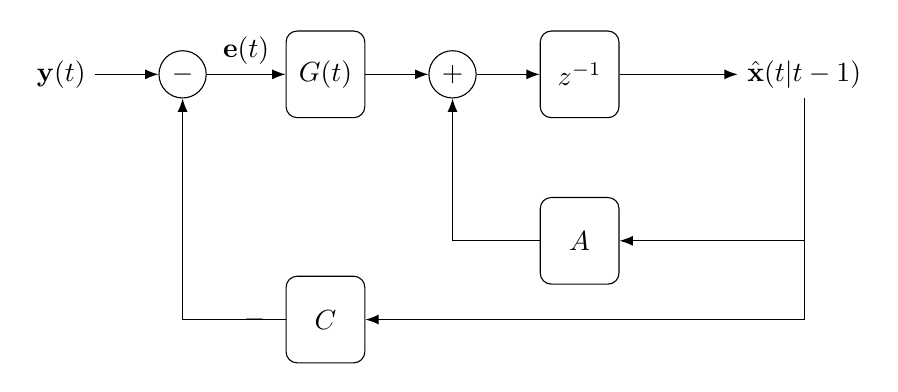
\begin{tikzpicture}[
    auto,
    >=Latex,
    node distance=1.8cm and 2.2cm,
    block/.style={draw, rectangle, rounded corners, minimum width=1cm, minimum height=1.1cm, align=center},
    sum/.style={draw, circle, inner sep=1pt, minimum size=6mm},
    input/.style={align=center},
    every path/.style={draw, -Latex}
]

% Nodes
\node[input] (y) {$\y(t)$};
\node[sum, right=.8cm of y] (innovsum) {$-$};
\node[block, right=1.0cm of innovsum] (gain) {$G(t)$};
\node[sum, right=.8cm of gain] (statesum) {$+$};
\node[block, right=.8cm of statesum] (z) {$z^{-1}$};
\node[input, right=1.5cm of z] (x) {$\xhat(t|t-1)$};

\node[block, below=1.0cm of z] (A) {$A$};
\node[block, below=2.0cm of gain] (C) {$C$};


% Connections
\path (y) -- (innovsum);
\path (innovsum) -- node {$\e(t)$} (gain);
\path (gain) -- (statesum);
\path (statesum) -- (z);
\path (C) -| node[pos=0.25, right] {$-$} (innovsum);
\path (A) -| node[pos=0.25, right] {} (statesum);
\path (x) |- node[pos=0.25, right] {} (A);
\path (x) |- node[pos=0.25, right] {} (C);
\path (z) -- (x);

\end{tikzpicture}

where the closed-loop dynamics is described by
$$
\Gamma(t) = A-G(t)C = F - K(t)C
$$
Hence its properties characterize the filter/predictor dynamics.
}

%--------------------------
\myframe{Filtered Estimates}{%

Similarly (for $S=0$ for simplicity)

\begin{align*}
    \xhat(t+1|t+1) &= A\xhat(t|t) + L(t+1)\left[\y(t+1)-CA\xhat(t|t)\right]\\
     P(t+1|t+1) &= \left[I-L(t+1)C\right]P(t+1|t)
\end{align*}

In this case the closed-loop dynamical behavior is described by

$$
\Gamma_{\rm filt}(t) = \left[I - L(t+1)C\right]A
$$

where before, with $S=0$, was $\Gamma_{\rm pred}(t)=A\left[I - L(t)C\right]$ which suggest
an almost identical asymptotic dynamic behavior.

\vspace{1cm}

\pause
\textit{Note that prediction and filtered estimates can directly be computed
from the original equations. It is sometimes convenient to get the explicit
expressions in order to better understand the role of the measurements in the
update.}

}

%--------------------------
\myframe{Kalman Filter with Input (part 1)}{
Reference model (with usual assumptions on noise and initial state):
%
\begin{align*}
    \x(t+1) &= A\x(t) + B\u(t) + \v(t) = F\x(t) + SR^{-1}\y(t) + B\u(t) + \verr(t)\\
    \y(t) &= C\x(t) + \w(t) + D\u(t)
\end{align*}


\pause
\textbf{Easy}: if $\u(t)$ \textbf{known and deterministic}
%
\begin{align*}
    \xhat(t+1|t) &= F\xhat(t|t) + SR^{-1}\y(t) + B\u(t)\\
    P(t+1|t) &= ...\ unchanged\\
    \e(t) &= y(t) - C\xhat(t|t-1) - D\u(t)
\end{align*}
%
$\Longrightarrow$ the deterministic input does not affect the uncertainty, only
the trajectory.

\pause
\medskip
\textbf{Harder}: \textit{but what if $\u(t)$ is a process?} E.g. a (linear) causal function ($H$) of
$\Hpast{t}(\y)$ plus a process uncorrelated from the entire noise ($\v, \w$)
history, say

$$
\u(t) = H(\y^t) + \r(t)
$$

\pause
In this case, even if $H\equiv 0$, it is in general not possible to assume
$\u(t)\perp\xzero$. Even if $\u(t)$ is observable, $\xhat$ based
on joint observations $(\y, \u)$ must be obtained by considering the joint state
model thus deriving augmented KF equations.

}

%--------------------------
\myframe{Kalman Filter with Input (part 2)}{

Assume the plant and input are described by

\begin{align*}
    &\begin{cases}
        \x_1(t+1) &= A\x_1(t) + B\u(t) + \v_1(t)\\
        \y(t) &= C \x(t) + \w_1(t)
    \end{cases}\\
    %
    &\begin{cases}
        \x_2(t+1) &= F\x_2(t) + G\y(t) + \v_2(t)\\
        \u(t) &= H\x_2(t) + J\y(t) + \w_2(t)
    \end{cases}
\end{align*}

\pause
This gives rise to the augmented state model to which standard KF can be applied

\begin{align*}
    \x(t+1) &=
    \underbrace{
        \begin{bmatrix}
            A+BJC & BH\\
            GC & F
        \end{bmatrix}
    }_{\mathcal A}
    \x(t)
    +
    \underbrace{
        \begin{bmatrix}
            \v_1(t) \\ \v_2(t)
        \end{bmatrix} +
        \begin{bmatrix}
            BJ & B\\
            G & 
        \end{bmatrix}
        \begin{bmatrix}
            \w_1(t) \\ \w_2(t)
        \end{bmatrix}
    }_{\overline{\v}(t)}\\
%
    \begin{bmatrix}
        \y(t)\\ \u(t)
    \end{bmatrix}
    &=
    \underbrace{
        \begin{bmatrix}
            C &  \\
            JC & H
        \end{bmatrix}
    }_{\mathcal C}
    \x(t) + 
    \underbrace{
        \begin{bmatrix}
            I & \\ J & I
        \end{bmatrix}
    }_{\mathcal{D}}
    \underbrace{
        \begin{bmatrix}
            \w_1(t) \\ \w_2(t)
        \end{bmatrix}
    }_{\w(t)}
\end{align*}

}

%--------------------------
\myframe{The Kalman Filter: information form}{%
    \begin{enumerate}
        \item Information variables
        \begin{itemize}
            \item Information matrix: $Y(t|t) \triangleq P(t|t)^{-1}$
            \item Information state: $\xi(t|t) \triangleq Y(t|t)\xhat(t|t)$
        \end{itemize}

        \pause
        \medskip
        \item A-priori estimates/predictions (temporal update)
        \begin{itemize}
            \item State:
                $
                \xi(t+1|t)
                =
                Y(t+1|t)
                \left(
                    F\,Y(t|t)^{-1}\xi(t|t)
                    +
                    SR^{-1}\y(t)
                \right)
                $
            \item Information matrix:
                $
                Y(t+1|t)
                =
                \left(
                    F\,Y(t|t)^{-1}F^T + \tilde{Q}
                \right)^{-1},
                \quad t\geq t_0
                $
        \end{itemize}

        \pause
        \medskip
        \item A-posteriori estimates/filters (measurement update)
        \begin{itemize}
            \item Information state:
                $
                \xi(t+1|t+1)
                =
                \xi(t+1|t) + C^T R^{-1}\y(t+1)
                $
            \item Information matrix:
                $
                Y(t+1|t+1)
                =
                Y(t+1|t) + C^T R^{-1} C
                $
        \end{itemize}

        \pause
        \medskip
        \item Initial conditions
        \begin{itemize}
            \item $Y(t_0|t_0-1)=\Pzero^{-1},\qquad \xi(t_0|t_0-1)=\Pzero^{-1}\muzero$
        \end{itemize}
    \end{enumerate}

    \pause
    where
    
    \begin{itemize}
        \item $Y(t|t-1)$, $Y(t|t)$: the prediction and filtering \underline{\textbf{information}} matrices
        \item $\xi(t|t-1)$, $\xi(t|t)$: the corresponding information states
        \item $\xhat(t|t)=Y(t|t)^{-1}\xi(t|t)$
    \end{itemize}
}

%--------------------------
\myframe{Kalman filter vs. Information filter}{%
    \begin{columns}[t]
        \column{0.49\textwidth}
        \textbf{Standard Kalman filter}
        \begin{itemize}
            \item Propagates
            \[
                \xhat(t|t),\quad P(t|t)
            \]
            \item Measurement update through
            \[
                \Lambda(t)=CP(t|t-1)C^T+R
            \]
            \item Gain computation required:
            \[
                L(t)=P(t|t-1)C^T\Lambda(t)^{-1}
            \]
            \item Natural for moderate state dimension and direct state reconstruction at each $t$
            \item Direct Covariance update
        \end{itemize}

        \column{0.49\textwidth}
        \textbf{Information filter}
        \begin{itemize}
            \item Propagates
            \[
                Y(t|t),\quad \xi(t|t)
            \]
            \item Measurement update is additive:
            \[
                Y^+ = Y^- + C^TR^{-1}C
            \]
            \[
                \xi^+ = \xi^- + C^TR^{-1}y
            \]
            \item No explicit Kalman gain
            \item Natural for multi-sensor fusion and sparse large-scale problems
            \item Particularly convenient when measurements are many and independent
        \end{itemize}
    \end{columns}

    \medskip

    \textbf{Key relation}
    \[
        Y(t|t)=P(t|t)^{-1},
        \qquad
        \xi(t|t)=Y(t|t)\xhat(t|t)
    \]
}

%--------------------------
\myframe{Why information form can be advantageous}{%
    \textbf{Example: fusion of many independent sensors}

    Assume $N$ sensors observe the same state:
    \[
        y_i(t)=C_i x(t) + v_i(t),
        \qquad
        v_i(t)\sim \mathcal N(0,R_i),
        \qquad i=1,\dots,N
    \]

    \pause
    \medskip
    \textbf{Standard Kalman filter}
    \begin{itemize}
        \item Meas. typically processed one by one, or stacked into one large vector
        \item This leads to repeated gain computations and innovation covariances
    \end{itemize}

    \pause
    \medskip
    \textbf{Information filter}
    \begin{itemize}
        \item Sensor contributes an additive information term (computed independently):
        \[
            Y(t|t)
            =
            Y(t|t-1)
            +
            \sum_{i=1}^{N} C_i^T R_i^{-1} C_i;
        \quad
            \xi(t|t)
            =
            \xi(t|t-1)
            +
            \sum_{i=1}^{N} C_i^T R_i^{-1} y_i(t)
        \]
        \item Very convenient for
        \begin{itemize}
            \item distributed sensor networks
            \item sparse estimation problems such as SLAM
        \end{itemize}
    \end{itemize}

    \pause
    \medskip
    \textbf{Main advantage}
    
    Updates are \underline{\textbf{simple accumulation of
information}}: more scalable and simpler.}



%--------------------------------
\subsection{Optimality and Asymptotic Theory}

%--------------------------------
\myframe{Cramer-Rao Lower Bound (CRLB) for KF}{
    
    \pause
    The CRLB defines the minimum theoretical variance of \underline{any
    unbiased estimator} of a \underline{deterministic parameter}, setting a
    fundamental limit on estimation precision. It is defined as the inverse of
    the Fisher information.

    \pause
    \medskip
    In the KF context, we deal with estimation of a \underline{time-varying
    random vector based on data and prior information}. Hence the relevant bound
    is what is usually referred to as the \textbf{posterior (Bayesian) CRLB}
    %
    $$
        \mathcal{I}(t|t) = -\E[\nabla_\x^2 \log p(\x(t)|\Hpast{t}(\y))\ |\ \Hpast{t}(\y)]\qquad \textnormal{Fisher Information Matrix}
    $$
    
    \medskip
    \begin{itemize}
        \pause
        \item For any unbiased estimator $\xhat_u(t|t)$ of $\x(t)$ from $\Hpast{t}(\y)$:
        \[
            \E[\xhat_u(t|t)-\x(t)] = 0,
            \qquad
            \Cov[\xhat_u(t|t)-\x(t)] \succcurlyeq \mathcal{I}(t|t)^{-1}
        \]
        %where $\mathcal{I}(t|t)$ is the Fisher information matrix.

        \pause
        \medskip
        \item Under the linear-Gaussian assumptions used for KF:
        \[
            \mathcal{I}(t|t)=Y(t|t)=P(t|t)^{-1} \quad \Longrightarrow \quad \Cov[\xhat_u(t|t)-\x(t)] \succcurlyeq P(t|t)
        \]
        and the Kalman filter attains the bound:
        \[
            \Cov[\xerr(t|t)]
            =
            \Cov[\x(t)-\xhat(t|t)]
            =
            P(t|t).
        \]
    \end{itemize}
}

%--------------------------
\myframe{Cramer-Rao limit (KF): proof of bound attainability}{
    Under the linear-Gaussian assumptions
    $\x(t)\,|\,\Hpast{t}(\y)\sim\mathcal N\!\left(\xhat(t|t),\,P(t|t)\right)$, where

    \[
        \xhat(t|t)=\Elin[\x(t)|\Hpast{t}(\y)]\equiv \E[\x(t)|\Hpast{t}(\y)]\quad (\textnormal{the KF})
    \]

    \medskip
    For any estimator $\xhat_u(t|t)$ based on $\Hpast{t}(\y)$, define
    \[
        d(t):=\xhat_u(t|t)-\xhat(t|t),
        \qquad
        \xerr(t|t):=\x(t)-\xhat(t|t).
    \]
    
    \medskip
    By the orthogonality principle of conditional expectation,
    % \[
    $\E\!\left[\xerr(t|t)\,d(t)^T\right]=0$.
    % \]

    \medskip
    Hence
    \begin{align*}
        \Cov[\x(t)-\xhat_u(t|t)]
        &= \Cov[\xerr(t|t)-d(t)]\\
        &= \Cov[\xerr(t|t)] + \Cov[d(t)]\\
        &= P(t|t) + \Cov[d(t)]
        \succcurlyeq P(t|t).
    \end{align*}

    Equality holds iff $\Cov[d(t)]=0$ (i.e., $d(t)=0$ a.s.), namely
    $\xhat_u(t|t)=\xhat(t|t)$
}

% %--------------------------
% \myframe{Asymptotic Behavior}{%

% \todo{add asymptotic behavior}

% }

%--------------------------
\myframe{Asymptotic Behavior: preliminaries}{%

  \textit{In the following we are going to see some results related to the
  \textbf{predictor} dynamics. The filtered estimates are intimately related and
  their behavior is essentially the same.}

  \pause
  \medskip
  \textit{Also, for the sake of compactness, in the next slides on the
  asymptotic behavior of the predictor we will resort to a slightly modified
  notation using subscripts, i.e.,} $\xhat(t|t-1)=\xhat_t$, $P(t|t-1)=P_t$.

  \pause
  \medskip
  \textit{Finally, we assume $S=0$, i.e., uncorrelated noises, to simplify the
  equations, i.e. $F=A$, $\tilde{Q}=Q$, $G_t=K_t=AL_t$, $\Gamma_t=A-K_tC$.} 

  \pause
  \medskip
  \medskip
  We recall the predictor dynamics equal to
  %
  \begin{align*}
    \xhat_{t+1} &= A\xhat_t + K_t\left[\y_t - C\xhat_t\right]\\
    P_{t+1} &=  A\left[P_t - P_tC^T\left(CP_tC^T + R\right)^{-1}CP_t \right]A^T + Q\\
    K_t &= AP_tC^T\left[CP_tC^T + R\right]^{-1}
  \end{align*}

}


%--------------------------
\myframe{Asymptotic Behavior: error dynamics}{%

  Also, defining the estimation error
  \[
    \e_t = \x_t - \xhat_t.
  \]
  %
  \pause
  After the update, the error dynamics are governed by
  %
  \begin{align*}    
   \e_{t+1} &= (A-K_tC)\e_t + \v_t - K_t \w_t\\
            &= \Gamma_t\e_t + \text{noise terms}
  \end{align*}

  \pause
  \vspace{.1cm}
  \textbf{Essentially, the covariance $P_t$ and, consequently, the gain $K_t$
  and closed-loop error $\Gamma_t$ dynamics are governed by the resolution of
  the discrete-time Riccati Equation (R.E.)}
  $$
  P_{t+1} =  A\left[P_t - P_tC^T\left(CP_tC^T + R\right)^{-1}CP_t \right]A^T + Q
  $$

  \medskip
  \pause
  Therefore:
  \begin{center}
  \emph{asymptotic filter behavior $\Longleftrightarrow$ asymptotic Riccati behavior.}
  \end{center}

  \medskip
  \pause
  \textit{Before looking at the behavior for the general case of non-stationary
  processes, we consider the stationary case.}

}

%--------------------------
\myframe{Asymptotic Behavior: the stationary case}{

\textit{In case of stationary processes and, in particular, asymptotically
stable systems, i.e., characterized by asymptotically stable state-space matrix
$A$ it is possible to state a strong direct result, connecting KF and
Wiener-Kolmogorov theories as well as the asymptotic stability of the filter.}

\pause
\medskip

\begin{exampleblock}{}
  If $A$ is asymptotically stable then
  $$
    \xhat_t = \Elin[\x_t|\y_0,\ldots,\y_t] \underset{t_0\to-\infty}{\longrightarrow} \xhat_t^\infty
  $$
  where $\xhat_t^\infty$ is the Wiener-Kolmogorov predictor of $\x_t$ based on
  the infinite past history of $\y$.
  Then, there exists
  $
  \lim_{t_0\to -\infty} P_t = P_\infty
  $
  with $P_\infty$ solution of the Algebraic Riccati Equation (ARE).
  The prediction satisfies
  \begin{align*}
    \xhat_{t+1}^\infty &= \Gamma_\infty\xhat_t^\infty + K_\infty\y_t \\ 
    K_\infty &= AP_\infty C^T\left[ CP_\infty C^T + R \right]^{-1} \\
    \Gamma_\infty &= A - K_\infty C 
  \end{align*}  
  And if $(\Gamma_\infty, K_\infty)$ is reachable, then $\Gamma_\infty$ is
  asymptotically stable.
\end{exampleblock}

}

%--------------------------
\myframe{Asymptotic Behavior: structural assumptions}{

  In the more general case of non-stationary processes ($A$ not asymptotically
  stable), the behavior is studied through the behavior of $P_t$ (i.e. of the RE)

  \medskip
  Yet, a couple of assumptions are needed\dots

  \pause
  \begin{block}{Detectability}
    The pair $(A,C)$ is \emph{detectable}: i.e., every unstable mode of $A$ is
    observable.
  \end{block}
  %
  \pause
  \begin{block}{Stabilizability}
    The pair $(A, Q^{1/2})$ is \emph{stabilizable}: i.e., every unstable mode of
    $A$ is reachable through the process noise channel.
  \end{block}
  %

  \pause
  These conditions (checked via PBH tests\footnote{\url{https://en.wikipedia.org/wiki/Hautus_lemma}}) are natural because:
  %
  \begin{itemize}
    \item unobservable unstable modes cannot be corrected from measurements,
    \item unreachable unstable modes create pathological Riccati behavior.
  \end{itemize}

  \pause
  \begin{alertblock}{}
    $R\succ0$, detect. of $(A,C)$, stab. of $(A,Q^{1/2})$ $\Longrightarrow$ $\exists !$ stabilizing steady-state $P_\infty$
  \end{alertblock}

}

% %--------------------------
% \myframe{Asymptotic Behavior: Discrete algebraic R.E.}{
%   A steady-state covariance $P_\infty$ must satisfy the fixed-point equation
%   \[
%   P = A P A^\top + GQG^\top - A P C^\top (CPC^\top + R)^{-1} C P A^\top.
%   \]
%   This is the \alert{filtering DARE}. Equivalently, the steady-state gain is
%   \[
%   K_\infty = P_\infty C^\top (C P_\infty C^\top + R)^{-1}
%   \]
%   for the filtered form, or the corresponding predictor gain depending on notation.

%   Important facts:
%   \begin{itemize}
%     \item the DARE can have multiple symmetric solutions,
%     \item only one is typically \emph{stabilizing},
%     \item the stabilizing solution is the one relevant for the asymptotic Kalman filter.
%   \end{itemize}
%   The associated steady-state error dynamics become time-invariant.
% }

% %--------------------------
% \myframe{Asymptotic Behavior: main convergence result $P$}{
%   Assume:
%   \[
%   R \succ 0, \qquad (A,C) \text{ detectable}, \qquad (A,GQ^{1/2}) \text{ stabilizable}.
%   \]
%   Then the Riccati recursion converges, for any initial covariance $P_0 \succeq 0$, to the unique stabilizing solution $P_\infty$ of the DARE:
%   \[
%   P_k \to P_\infty.
%   \]
%   Consequently,
%   \[
%   K_k \to K_\infty.
%   \]
%   Moreover, the corresponding closed-loop estimation dynamics are asymptotically stable:
%   \[
%   \rho\bigl(A - K_\infty C\bigr) < 1
%   \]
%   (or the equivalent predictor-form matrix under the adopted indexing convention).

%   Interpretation:
%   \begin{itemize}
%     \item after transients, the filter ``forgets'' the initial covariance,
%     \item the gain becomes constant,
%     \item the estimation error reaches a stationary covariance regime.
%   \end{itemize}
% }

%--------------------------
\myframe{Asymptotic Behavior: fundamental theorem of KF theory}{

  \begin{exampleblock}{}
    Necessary and sufficient condition for:
    
    \begin{itemize}
      \item $\exists !$ a symmetric $P_\infty$ solution of the A.R.E.
      $$
      P = APA^T - APC^T(CPC^T + R)^{-1}CPA^T + Q
      $$
      \item the solution $P_\infty$ is stabilizing
      \item $\lim_{t\to\infty} P_t = P_\infty\quad \forall$ initial symmetric
      positive semidefinite $P_0$ 
    \end{itemize}

    is that $(A,C)$ being detectable and $(F,Q^{1/2})$ being stabilizable.
  \end{exampleblock}

  \pause
  \medskip
  Interpretation:
  \begin{itemize}
    \item after transients, the filter ``forgets'' the initial covariance,
    \item the gain becomes constant,
    \item the estimation error reaches a stationary covariance regime.
  \end{itemize}

}

%--------------------------
\myframe{Asymptotic Behavior: steady-state KF}{
  
  Analogously to the stationary
  case, once $P_k$ and $K_k$ have converged, one can replace the time-varying
  filter by the constant-gain filter
  \begin{align*}
    \xhat_{t+1|t} &= A \xhat_{t|t},\\
    \xhat _{t+1|t+1} &= \xhat_{t+1|t} + K_\infty (\y_{t+1} - C \xhat_{t+1|t}).
  \end{align*}

  \pause
  Equivalently, for the predictor
  \[
  \xhat_{t+1|t} = (A-K_\infty C)\xhat_{t|t-1} + K_\infty y_{t}.
  \]

  \pause
  Advantages of the constant-regime filter:
  \begin{itemize}
    \item lower online computational cost,
    \item simpler implementation in embedded systems,
    \item explicit LTI error dynamics,
    \item same asymptotic performance as the full Kalman filter.
  \end{itemize}

  Hence, for time-invariant models, the practical end-point is often a
  \emph{steady-state Kalman filter}.

}

%--------------------------
\myframe{Asymptotic Behavior: transient vs asymptotic phases}{
  Two phases are usually observed:
  
  \pause
  \begin{block}{Transient phase}
    $P_k$ depends on $P_0$ and the gain $K_k$ varies significantly. The filter is learning how much to trust model vs measurements.
  \end{block}

  \pause
  \begin{block}{Asymptotic phase}
    $P_k \approx P_\infty$ and $K_k \approx K_\infty$. The filter has entered a stationary regime.
  \end{block}
  
  \pause
  The tuning parameters shape this regime:
  \[
  Q \uparrow\ \Rightarrow\ K_\infty \uparrow \quad \text{(more trust in measurements)},
  \]
  \[
  R \uparrow\ \Rightarrow\ K_\infty \downarrow \quad \text{(more trust in the model)}.
  \]

  \pause
  The asymptotic gain is the precise mathematical embodiment of the
model/measurement tradeoff. }

%--------------------------
\myframe{Asymptotic Behavior: continuous-time counterpart}{
  For the continuous-time model
  \[
  \dot x = A x + G w, \qquad y = Cx + v,
  \]
  with white noises of intensities $Q$ and $R$, the covariance satisfies the differential Riccati equation
  \[
  \dot P = A P + P A^\top + GQG^\top - P C^\top R^{-1} C P.
  \]
  \pause
  At steady state, $P_\infty$ solves the continuous algebraic Riccati equation (CARE)
  \[
  A P + P A^\top + GQG^\top - P C^\top R^{-1} C P = 0.
  \]
  \pause
  Under the analogous detectability/stabilizability assumptions,
  \[
  P_t \to P_\infty,
  \qquad
  K_t=P_tC^\top R^{-1} \to K_\infty = P_\infty C^\top R^{-1}.
  \]
  \pause
  The constant-regime filter is then the steady-state Kalman--Bucy filter.
}

%--------------------------
\myframe{Asymptotic Behavior: take-away results}{
  \begin{enumerate}
    \pause
    \item The asymptotic behavior of the Kalman filter is governed by a R.E.
    \pause 
    \item Under
    \[
    (A,C) \text{ detectable}, \qquad (A,Q^{1/2}) \text{ stabilizable}, \qquad R\succ0,
    \]
    the Riccati recursion converges to a unique stabilizing solution $P_\infty$.
    \pause  
    \item The filter gain converges: $K_k \to K_\infty$
    \pause
    \item The estimation error covariance converges: $P_k \to P_\infty$
    \pause
    \item The asymptotic filter becomes a constant-gain linear filter with the same steady-state performance as the full time-varying Kalman filter.
  \end{enumerate}

  \vspace{.6cm}
  \texttt{4\_asymptotic\_behavior.ipynb}
}



\section{Nonlinear Theory}
\sectionframe{3}{Nonlinear Theory}


%--------------------------
\myframe{Linear vs Nonlinear Kalman Filtering}{%
    \begin{itemize}
        \item \textbf{Linear Kalman Filter (KF)}: Assumes linear system dynamics and measurement models.

        \pause
        \medskip
        \item \textbf{Nonlinear versions}:
        \begin{itemize}
            \item \textbf{Extended Kalman Filter (EKF)}: Linearizes nonlinear models using Taylor series expansion.
            \item \textbf{Unscented Kalman Filter (UKF)}: Uses deterministic sampling to capture mean and covariance of nonlinear transformations.
            \item \textbf{Other variants}: E.g. Particle Filters (PFs), use random sampling to approximate any underlying distribution.
        \end{itemize}
    \end{itemize}

    \pause
    \medskip
    \centering
    \begin{tabular}{l|lp{2cm}p{4cm}}
        \textbf{Estimator} & \textbf{Model} & \textbf{Assumed Distribution} & \textbf{Computational Cost}\\
        \hline
        \hline
        KF & Linear  & Gaussian  & Low \\
        \hline
        EKF & Locally Linear  & Gaussian  & Low/Medium (depends on Jacobians) \\
        \hline
        UKF & Nonlinear  & Gaussian  & Medium \\
        \hline
        PFs & Nonlinear  & Arbitrary  &  High 
    \end{tabular}

}


%-------------------------------------------------------------------------------
\subsection{Extended Kalman Filter}

%--------------------------
\myframe{Extended Kalman Filter (EKF): essentials and notation}{%
    \begin{itemize}
        \item Linearizes nonlinear functions $f(x,u)$ and $h(x)$ around current estimate.
        \item Same equations as linear KF, but with linearized matrices.
        \item Limitations: Linearization errors, Jacobian computation.
    \end{itemize}

    \pause
    \medskip
    Consider a discrete-time\footnote{Here we make use of $k$ or $t_k$ to denote
    discrete-time instants since $t$ will later be used to denote continuous
    time.} non-linear state model of the form

    \begin{align*}
        \x(k+1) &= f(\x(k), \u(k)) + \v(k),\quad \v\sim\N(0,Q)\\
        \y(k)   &= h(\x(k)) + \w(k),\quad \w\sim\N(0,R)
    \end{align*}

    under the usual assumptions $\v\perp\w\perp\xzero$,
    \pause
    and denote the Jacobian matrices

    $$
        F_k = \left.\frac{\partial f}{\partial x}\right|_{\hat{x}_{k|k}}\qquad
        H_k = \left.\frac{\partial h}{\partial x}\right|_{\hat{x}_{k+1|k}}
    $$
}


%--------------------------
\myframe{EKF: discrete-time equations}{%

\begin{enumerate}
    \item Prior estimates
        \begin{itemize}
            \item State: $\xhat(k+1|k) = f(\xhat(k|k), \u(k))$
            \item Variance: $P(k+1|k) = F_kP(k|k)F_k^T + Q$,
        \end{itemize}

    \pause
    \medskip
    \item Measurement update
        \begin{itemize}
            \item State: $\xhat(k+1|k+1) = \xhat(k+1|k) + L(k+1)\left[\y(k+1)-h\left(\xhat(k+1|k)\right)\right]$
            \item Variance: $P(k+1|k+1) = (I - L(k+1) H_k) P(k+1|k)$ 

            \medskip
            \item $L(k+1) = P(k+1|k) H_k^T \Lambda(k+1)^{-1}$
            \item $\Lambda(k+1) = H_kP(k+1|k)H_k^T + R$ 
        \end{itemize}

    \pause
    \medskip
    \item Initial conditions
        \begin{itemize}
            \item $\xhat(0|-1)=\E[\x(t_0)]$
            \item $P(0|-1)=\Var[\x(t_0)]$  
        \end{itemize}
\end{enumerate}

\pause
\medskip
Nonlinearity used to properly propagate the prior estimate and the measurement
model to compute the pseudo innovation.

}

%--------------------------
\myframe{EKF: generalization - continuous-discrete equations}{%

    The EKF is also used in more general setups of continuous-discrete systems.

    \pause
    \medskip
    Consider a continuous-time state-model with sampled
    measurements at discrete instants $t_k$ (possibly non uniform)
    %
    \begin{align*}
        \dot{\x}(t) &= f(\x(t)) + \xi(t)\\
        \y(t_k) &= h(\x(t_k)) + \w(t_k) 
    \end{align*}
    %
    being $\xi$ white noise of intensity $Q\geq0$; $\w(t_k)$ white of variance
    $R>0$ and $\{\xi(t)\}\perp\{\w(t_k)\}\perp\x(t_0)$. $f,h\in\C^1$.
    %

    \pause
    Let $\Phi(t,s,\overline{\x})$ be the fundamental matrix\footnote{Matrix
    satisfying the Volterra equation which, for constant F, equals
    $\Phi(t,s)=e^{F(t-s)}$.} associated to the time-varying linear system
    $\dot{\z}=F(\overline{\x}(t))\z$ where $F(\overline{\x}(t))= \frac{\partial
    f}{\partial x}|_{\x=\overline{\x}(t)}$ and define
    $$
        Q(t_k) := \int_{t_k}^{t_{k+1}} \Phi(t_{k+1},s,\overline{\x})Q\Phi(t_{k+1,s},\overline{\x})^T ds
    $$

    Under these conditions, the equations generalize as follows.

}

%--------------------------
\myframe{EKF: generalization - continuous-discrete equations}{%
    
    \begin{enumerate}
        \setcounter{enumi}{0}
        \item Prior estimates
    \end{enumerate}
    \begin{itemize}
        \item State:
            \begin{itemize}
                \item Resolve $\dot{\overline{\x}}(t)=f(\overline{\x}(t))$, $t\in[t_k,t_{k+1}]$, $\overline{\x}(t_k)=\xhat(k|k)$ 
                \item Set $\xhat(k+1|k)=\overline{\x}(t_{k+1})$
            \end{itemize}
        \item Variance: 
            \begin{itemize}
                \item $P(k+1|k) = \Phi(k|k)P(k|k)\Phi(k|k)^T + Q(k)$, $\Phi(k|k):=\Phi(k+1,k,\xhat(k|k))$
                \item Alternative CT Riccati: $\dot{P}(t) = F(t)P(t) + P(t)F(t)^T + Q(t)$
            \end{itemize}
    \end{itemize}

    \pause
    \begin{enumerate}
        \setcounter{enumi}{1}
        \item Measurement update
    \end{enumerate}
    \begin{itemize}
        \item State:
            \begin{itemize}
                \item $\xhat(k+1|k+1) = \xhat(k+1|k) + L(k+1)\left[\y(k+1)-h\left(\xhat(k+1|k)\right)\right]$
                \item $L(k+1) = P(k+1|k) H(k+1|k)^T \Lambda(k+1)^{-1}$
                \item $\Lambda(k+1) = H(k+1|k)P(k+1|k)H(k+1|k)^T + R$ 
                \item $H(k+1|k) := H(\xhat(k+1|k)) = \frac{\partial h}{\partial x}|_{\x=\xhat(k+1|k)}$
            \end{itemize}
        \item Variance: $P(k+1|k+1) = (I - L(k+1) H(k+1|k)) P(k+1|k)$ 
    \end{itemize}

    with initial conditions $\xhat(0,-1)=\E[\x(t_0)], P(0|-1)=\Var[\x(t_0)]$

}


%--------------------------
\myframe{EKF: observations}{%

\begin{itemize}
    \item The linearized model is used only to compute $L(k)$.
    
    \pause
    \item The statistical interpretation of $\xhat(k+1|k)$ and $\xhat(k|k)$ can
    not in general be drawn being both non-linear functions of the data.

    \pause
    \item The algorithm is much more computationally intense. It requires
    computation of $H$ and $\Phi$ at every step, hence $L$ cannot be precomputed
    offline.
    
    \pause
    \item Adding a linear additive term $B\u(t)$ for an input component does not
    essentially complicate the filter equations.
\end{itemize}

\pause
To avoid explicit integration, when the signals
are sufficiently slow w.r.t. the sampling time, a full DT
scheme is used, by discretizing the CT dynamics, e.g.,
%
$$
\x(k+1) = \hat{f}_k(\x(k)) \overset{Euler}{=} \x(k) + (t_{k+1}-t_k)f(\x(k))
$$
also used to propagate the prior estimated state in the filter equations
%
$$
\xhat(k+1|k) = \hat{f}_k(\xhat(k|k))
$$

All other equations remain the same assuming now $\Phi(k|k)=\frac{\partial \hat{f}_k}{\partial x}|_{\x=\xhat(k|k)}$.

}


%-------------------------------------------------------------------------------
\subsection{Unscented Kalman Filter}

%--------------------------
\myframe{Unscented Kalman Filter (UKF)}{%
    \begin{itemize}
        \item Uses sigma points to capture higher-order moments: for any random
        vector $\x$, sigma points are a set of any $N$ vectors satisfying:
        \begin{itemize}
            \item first order: weighted average of points corresponds to $\E[\x]$
            \item second order: weighted average of points covariance corresponds to $\Var[\x]$ 
        \end{itemize}
        The critical point is to find the right choice of weights: for this
        standard approaches exists.

        \pause
        \item UKF usually generates $2n+1$ sigma points where $n$ is state dimension.

        \pause
        \item Propagates sigma points through nonlinear functions.
        
        \pause
        \item Reconstructs mean and covariance from transformed sigma points.
        
        \pause
        \item \textit{Main Advantages}:
        \begin{itemize}
            \item No Jacobian required wrt EKF
            \item  better handling of nonlinearities since $P$ is estimated
            considering nonlinear transforms.
        \end{itemize}
    \end{itemize}

\pause
\medskip
\textit{UKF equations are not difficult but heavy in notation. We'll see them in
code rather than on slides.}

}

%--------------------------
\myframe{UKF: graphical representation}{

\centering
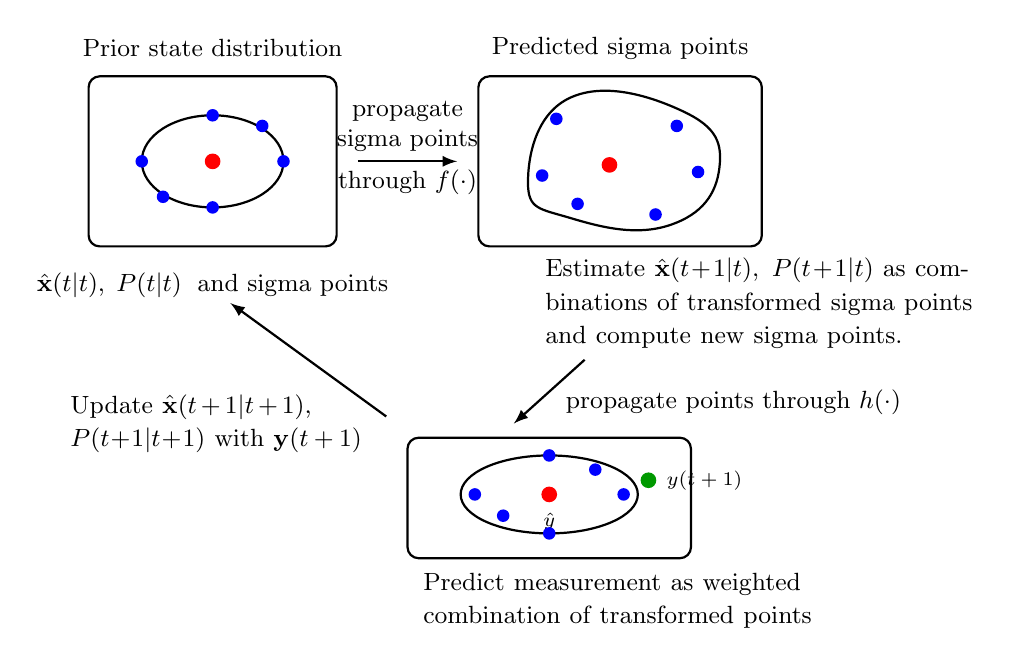
\begin{tikzpicture}[scale=0.9, >=latex]

    % Styles
    \tikzstyle{statecloud}=[draw, rounded corners, thick]
    \tikzstyle{arrow}=[->, thick]
    \tikzstyle{sigmapt}=[circle, fill=blue, inner sep=1.6pt]
    \tikzstyle{meanpt}=[circle, fill=red, inner sep=2pt]

    %-------------------------
    % Prior state box
    %-------------------------
    \draw[statecloud] (0,0.3) rectangle (3.5,2.7);
    \node at (1.75,3.1) {\small Prior state distribution};
    \node at (1.75,-0.25) {\small $\xhat(t|t),\;P(t|t)$\; and sigma points};

    % Prior ellipse
    \draw[thick] (1.75,1.5) ellipse (1.0 and 0.65);

    % Prior sigma points
    % \node[meanpt,label=below:{\scriptsize $\hat x$}] at (1.75,1.5) {};
    \node[meanpt] at (1.75,1.5) {};
    \node[sigmapt] at (2.75,1.5) {};
    \node[sigmapt] at (0.75,1.5) {};
    \node[sigmapt] at (1.75,2.15) {};
    \node[sigmapt] at (1.75,0.85) {};
    \node[sigmapt] at (2.45,2.0) {};
    \node[sigmapt] at (1.05,1.0) {};

    %-------------------------
    % Propagation arrow
    %-------------------------
    \draw[arrow] (3.8,1.5) -- (5.2,1.5);
    \node at (4.5,2.2) {\small propagate};
    \node at (4.5,1.8) {\small sigma points};
    \node at (4.5,1.2) {\small through $f(\cdot)$};

    %-------------------------
    % Predicted state box
    %-------------------------
    \draw[statecloud] (5.5,0.3) rectangle (9.5,2.7);
    \node at (7.5,3.1) {\small Predicted sigma points};
    \node[text width=5.5cm] at (9.5,-0.5) {%
        \small Estimate $\xhat(t\!+\!1|t),\;P(t\!+\!1|t)$ as
        combinations of transformed sigma points and
        compute new sigma points.
        };

    % Nonlinear transformed cloud
    \draw[thick] plot[smooth cycle, tension=0.8] coordinates {
        (6.2,1.2) (6.8,2.4) (8.4,2.2) (8.9,1.4) (8.2,0.6) (6.8,0.7)
    };

    % Predicted sigma points
    % \node[meanpt,label=below:{\scriptsize $\hat x^-$}] at (7.35,1.45) {};
    \node[meanpt] at (7.35,1.45) {};
    \node[sigmapt] at (6.6,2.1) {};
    \node[sigmapt] at (8.3,2.0) {};
    \node[sigmapt] at (8.6,1.35) {};
    \node[sigmapt] at (8.0,0.75) {};
    \node[sigmapt] at (6.9,0.9) {};
    \node[sigmapt] at (6.4,1.3) {};

    %-------------------------
    % Measurement projection arrow
    %-------------------------
    \draw[arrow] (7,-1.3) -- (6,-2.2);
    \node at (9.1,-1.9) {\small propagate points through $h(\cdot)$};

    %-------------------------
    % Measurement box
    %-------------------------
    \draw[statecloud] (4.5,-4.1) rectangle (8.5,-2.4);
    % \node at (7.5,-1.95) {\small Predicted measurement};
    \node[text width=5cm] at (7.5,-4.7) {\small Predict measurement as weighted combination of transformed points};
    % \node at (7.5,-5.3) {\small $\hat y(t\!+\!1),\;S(t\!+\!1)$};

    % Measurement ellipse
    \draw[thick] (6.5,-3.2) ellipse (1.25 and 0.55);

    % Measurement sigma points
    \node[meanpt,label=below:{\scriptsize $\hat y$}] at (6.5,-3.2) {};
    \node[sigmapt] at (7.55,-3.2) {};
    \node[sigmapt] at (5.45,-3.2) {};
    \node[sigmapt] at (6.5,-2.65) {};
    \node[sigmapt] at (6.5,-3.75) {};
    \node[sigmapt] at (7.15,-2.85) {};
    \node[sigmapt] at (5.85,-3.5) {};

    % Actual measurement
    \node[circle, fill=green!60!black, inner sep=2pt,
          label=right:{\scriptsize $y(t+1)$}] at (7.9,-3) {};

    %-------------------------
    % Update arrow back
    %-------------------------
    % \draw[arrow] (9.9,-1.0) .. controls (11.0,-1.0) and (11.0,2.2) .. (9.7,2.2);
    \draw[arrow] (4.2,-2.1) -- (2,-0.5);

    % Posterior label inside predicted box
    \node[text width=3.7cm] at (1.8,-2.2) {\small Update $\xhat(t\!+\!1|t\!+\!1)$, $P(t\!+\!1|t\!+\!1)$ with $\y(t+1)$};

\end{tikzpicture}

}

%-------------------------------------------------------------------------------
\subsection{Particle Filters}

%--------------------------
\myframe{Particle Filters (PFs)}{

Particle Filters are a family rather than a single estimation algorithm.

\medskip
General idea:
\begin{itemize}
    \item use many samples/particle
    \item use random sampling to approximate any underlying distribution
    \item often exploit a \textit{genetic} approach consisting of a
    selection/updating step alternate with a mutation/prediction step
\end{itemize}

\medskip
Common implementations are:
\begin{itemize}
    \item Markov Chain Monte Carlo
    \item Sequential Importance Sampling (SIS)
    \item Sequential Importance Resampling (SIR)
\end{itemize}

}

\section{Adds-on}
\sectionframe{3}{Adds-on}

% --------------------------
\subsection{Filter Tuning}

% --------------------------
\myframe{A Practical Recipe for Tuning a Kalman Filter (part 1)}{

\textbf{Goal:} essentially, tune the two covariances that matter most:
\[
Q \quad\text{(process noise)} \qquad R \quad\text{(measurement noise)}
\]

\pause
\medskip
\textbf{1. Estimate measurement noise $R$ from real data}
\begin{itemize}
    \item Hold the system still or run in a regime with known truth
    \item Compute sample covariance of sensor error
\end{itemize}
\[
    R \approx \mathrm{cov}(y_k - y^{\mathrm{true}}_k)
    \quad \text{or approximately} \quad
    R \approx \mathrm{cov}(y_k - \bar y)
\]

\pause
\medskip
\textbf{2. Parameterize process noise \(Q\) simply}

Start with simple diagonal $Q$ and then move towards $Q = \alpha Q_0$, where
\(Q_0\) encodes relative trust between states and \(\alpha\) is one scalar to
tune.

\pause
\medskip
\textbf{3. Check the innovations}
\[
\nu_k = y_k - H\hat x_k^-,
\qquad
S_k = H P_k^- H^\top + R
\]
A good filter has innovations that are approximately white, zero-mean, and with
the expected size (covariance close to \(S_k\)).

}

% --------------------------
\myframe{A Practical Recipe for Tuning a Kalman Filter (part 2)}{

\textbf{4. Tune using observed behavior}
\begin{center}
    \begin{tabular}{ll}
        \textbf{Symptom} & \textbf{Adjustment} \\
        \hline
        Estimate too noisy & increase \(R\) or decrease \(Q\) \\
        Estimate too sluggish & increase \(Q\) or decrease \(R\) \\
        Bias / drift not tracked & increase \(Q\) on bias states \\
    \end{tabular}
\end{center}

\pause
\medskip
\textbf{Best practical rule:} fix \(R\) from measurements, then tune only \(Q\)
until the filter is as fast as possible without visibly fitting noise.

\medskip
\begin{exampleblock}{Example sweep}
    \texttt{for alpha in [1e-3, 1e-2, ..., 1e3]:}\\
    \texttt{\hspace{.5cm} Q = alpha * Q0}\\
    \texttt{\hspace{.5cm} run filter}\\
    \texttt{\hspace{.5cm} inspect innovation variance + tracking lag}
\end{exampleblock}

}



%--------------------------
\subsection{Kalman Smoother}

\myframe{Fixed-Interval Rauch-Tung-Striebel Smoother}{%

\textbf{Objective of smoothing}:
\begin{itemize}
    \item Fixed-lag: provide an almost real-time (slightly delayed) improved
    estimate at $k-N$ using a sliding window of measurements up to $k$.
    \item Fixed-interval: provide the best estimate using all available
    measurements up to a certain instant $n$.
\end{itemize}

\pause
\medskip
The RTS smoother\footnote{There are also other smoother implementation e.g., the Modified
Bryson-Frazier, which we are not going to cover.} consists of:
\begin{itemize}
    \item forward pass: exactly equal to the standard KF equations to compute
    $\xhat(k|k-1)$, $\xhat(k|)$, $P(k|k-1)$ and $P(k|k)$.

    \pause
    \item backward pass: compute the \textit{smoothed} estimates $\xhat(k|n)$,
    $P(k|n)$ via
    \begin{itemize}
        \item $\xhat(k|n) = \xhat(k|k) + C_k\left(\xhat(k+1|n) - \xhat(k+1|k)\right)$
        \item $P(k|n) = P(k|k) + C_k\left( P(k+1|n) - P(k+1|k) \right)C_k^T$  
        \item $C_k = P(k|k)F^TP(k+1|k)^{-1}$
    \end{itemize}
\end{itemize}

\pause
\medskip
Note that, conversely to fixed-lag smoothers, fixed-interval are
\textbf{offline} algorithms as they require all future measurements up to $n$.

}


%--------------------------
\subsection{Control perspective: LQG}

%--------------------------
\myframe{LQG control and its connection to KF}{%

    \textbf{Problem setup (stochastic optimal control)}
    \[
    x_{t+1} = A x_t + B u_t + w_t,\quad
    y_t = C x_t + v_t,\quad
    w_t \sim \mathcal N(0,Q),\quad v_t \sim \mathcal N(0,R)
    \]

    \medskip

    \textbf{Objective (LQG cost):}
    $
    J = \mathbb E\!\left[\sum_{t=0}^{T}
    x_t^T Q_x x_t + u_t^T R_u u_t
    \right]
    $

    \medskip

    \textbf{Key result (Separation principle)}: \boxed{\text{Optimal control = LQR + KF}}

    \medskip
    \begin{itemize}
        \item \textbf{State estimation (Kalman filter)}: $\xhat(t|t) = \E[\x_t \mid \Hpast{t}(\y)]$

        \item \textbf{Control law (LQR)}: $u_t = -K_t \xhat(t|t)$ (Controller uses $\xhat$, not $\x$)
    \end{itemize}

    \medskip

    \textbf{Dual Riccati equations} (forward + backward)

    \begin{itemize}
        \item KF covariance:
        $
        P_{t+1} = A P_t A^T + Q - A P_t C^T (C P_t C^T + R)^{-1} C P_t A^T
        $

        \item LQR cost2go:
        $
        S_t = A^T S_{t+1} A + Q_x - A^T S_{t+1} B (B^T S_{t+1} B + R_u)^{-1} B^T S_{t+1} A
        $
    \end{itemize}

    \vspace{-0.1cm}

    % \medskip

    % \textbf{KF vs LQR (duality)}

    % \[
    % \boxed{
    % \begin{array}{c|c}
    % \text{Estimation (KF)} & \text{Control (LQR)}\\
    % \hline
    % A,\;C & A^T,\;B^T \\
    % Q,\;R & Q_x,\;R_u \\
    % P_t & S_t \\
    % \text{Kalman gain} & \text{feedback gain}
    % \end{array}
    % }
    % \]

    % \medskip

    % \textbf{Interpretation}

    % \begin{itemize}
    %     \item KF = optimal \emph{information extraction}
    %     \item LQR = optimal \emph{control action}
    %     \item LQG = optimal closed-loop system under uncertainty
    % \end{itemize}

    \begin{columns}[t]
        %---------------- LEFT COLUMN ----------------
        \column{0.52\textwidth}
        \vspace{-0.3cm}
        %
        \[
        \boxed{
        \begin{array}{c|c}
        \text{KF (estimation)} & \text{LQR (control)}\\
        \hline
        A,\;C & A^T,\;B^T \\
        Q,\;R & Q_x,\;R_u \\
        P_t & S_t \\
        K_t^{\text{KF}} & K_t^{\text{LQR}}
        \end{array}
        }
        \]

        %---------------- RIGHT COLUMN ----------------
        \column{0.48\textwidth}

        \textbf{Interpretation}

        \begin{itemize}
            \item KF: optimal \emph{information extraction}
            \item LQR: optimal \emph{control action}
            \item LQG: optimal closed-loop system
        \end{itemize}

    \end{columns}

}

%--------------------------
\myframe{Additional resources}{

\begin{itemize}
    \item https://github.com/mintisan/awesome-kalman-filter?tab=readme-ov-file
    \item https://github.com/rlabbe/Kalman-and-Bayesian-Filters-in-Python
    \item https://kalmanfilter.net/
\end{itemize}
}


%--------------------------
\myframe{}{
\centering
\LARGE
End! Thank you!
}

\end{document}
